\documentclass[10pt]{article}
\usepackage[utf8]{inputenc}
\usepackage[T1]{fontenc}
\usepackage[a4paper,margin=2.1cm]{geometry}
\usepackage{amsmath,amssymb}
\usepackage{mathptmx}
\usepackage{booktabs}
\usepackage{array}
\usepackage{graphicx}
\usepackage{caption}
\usepackage{float}
\usepackage[hidelinks]{hyperref}
\usepackage{ragged2e}

% ---- Nature-style look -------------------------------------------------
\setlength{\parindent}{0pt}
\setlength{\parskip}{4pt plus 1pt}
\renewcommand{\baselinestretch}{1.06}
% superscript reference markers, e.g. "...errors\textsuperscript{\ref{BP86}}."
\newcommand{\natref}[1]{\textsuperscript{\ref{#1}}}
% reference list labels "1." instead of "[1]"
\makeatletter
\renewcommand{\@biblabel}[1]{#1.}
\makeatother
% section headings: bold, sentence case, unnumbered (Nature style)
\makeatletter
\renewcommand\section{\@startsection{section}{1}{\z@}%
  {-14pt plus -2pt minus -2pt}{6pt plus 2pt}%
  {\normalfont\bfseries\large}}
\renewcommand\subsection{\@startsection{subsection}{2}{\z@}%
  {-10pt plus -2pt minus -2pt}{4pt plus 1pt}%
  {\normalfont\bfseries\normalsize}}
\makeatother
% caption style: bold "Figure N |" prefix (Nature style)
\captionsetup{labelformat=empty, font={small}, skip=4pt}
\newcommand{\figcap}[2]{\caption{\textbf{#1 |} #2}}
% compact tables
\newcolumntype{L}[1]{>{\RaggedRight\arraybackslash}p{#1}}
\newcolumntype{C}[1]{>{\centering\arraybackslash}p{#1}}

\begin{document}
\begin{center}
{\Large\bfseries Morphogenetic Bi-Modal Networks:\\
Gradient-Free System Identification\\
and Computation through Self-Organized 3D Angulation}
\vspace{0.5em}
{\small Preprint --- every quantitative claim is the measured output of the
accompanying experiment suite (\texttt{results.json}, \texttt{ablation.json},
\texttt{scaling.json}).}
\end{center}
\vspace{0.6em}

\begin{abstract}
The training loop of deep learning rests on two assumptions that the physics of
biological tissue and of ultra-low-power hardware both violate: a global scalar loss and
a global computational graph through which gradients flow. Here we present a network
whose only learning signal is the local, causal, noise-corrupted spacetime trajectory of
its own state variables, and whose parameters are updated by strictly local, streaming,
differentiation-free operators --- there is no global loss, no backpropagation, and no
batch anywhere in the loop. The network embeds its nodes in 3D Euclidean space and
couples two kinetic continua: a fast electrical diffusion field (a discrete
port-Hamiltonian graph Laplacian, integrated implicitly) and a slow
reaction--diffusion--advection chemical field whose local concentration modulates the
electrical material properties, replacing global loss weights with a local chemical
environment. Identification proceeds through a spacetime weak form: every governing
equation is integrated against a one-pole IIR test function so that time derivatives are
transferred from the noisy data onto the analytic filter by integration by parts,
replacing the $2/\Delta t^2$ noise amplification of finite differences with
$\lambda^2$. Each node fits its local flux law with per-node recursive least squares.
In parallel, a slow morphogenesis layer \emph{rotates} each node's 3D structural vector
--- learning acts on angles, not on scalar weights --- and the resulting shape feeds back
into the conductivity, closing a fully local loop.

Measured on a 49-node material under continuous chaotic excitation, 5\% observational
noise, and abrupt regime-switching drift (15 seeds): the streaming identifier reaches a
held-out law-fit error \textbf{11.8$\times$ lower than a frozen global batch
least-squares estimator in the correct model class}, \textbf{8.9$\times$ lower than the
best streaming-global RLS estimator} (isolating per-node locality itself as the source
of the advantage), and \textbf{15.3$\times$ lower than an identical finite-difference
identifier}, while holding \textbf{589$\times$ less runtime memory} and converging in
$0.24 \pm 0.08$~s (15/15 seeds). The self-organized shape is a \emph{readable and
functional representation}: the geometric coupling read off the angles alone correlates
with the full material law at $r = 0.64$, versus $r = 0.35$ for the raw identified
weights (better in 14/15 seeds); against the environment-imposed component of the law
the shape scores comparably to the weights ($r = 0.33$ vs $0.39$), showing that its
interpretability is \emph{constructive} --- the shape constitutes part of the mechanism
rather than mirroring hidden weights. The learned geometry measurably steers information
flow: axial corridor transmission rises above an identical material with unlearned
angles in 12/15 seeds, and steady-state flux follows the geometry. Ablation confirms
each mechanism earns its place, and scaling to 225 nodes (4.6$\times$ more material)
preserves the identification advantage and \emph{improves} the coherence of
self-organization (wind alignment $0.71 \to 0.87$) under constant excitation power
density. With a sparse, warm-started conjugate-gradient plant solver --- the
relaxation a physical material actually performs, exact to $10^{-9}$ --- the same
network runs at \textbf{$10^4$ nodes (44$\times$ more material than the
dense-solve table)} with the identification advantage and shape readability intact
($r \approx 0.63$ at every size), a memory advantage that \emph{grows} with scale
(${\sim}240\times \to {\sim}630\times$), and sublinear per-node cost. Finally, on
\emph{two} real signals that no part of the pipeline generated --- the 277-year
SILSO sunspot record and the 78-year NINO3.4 El Ni\~no SST record --- the same
frozen weak-form identifier generalizes to unseen decades at \textbf{${\sim}500\times$
(sunspot) and ${\sim}22\times$ (ENSO) lower holdout error than finite-difference
identification}, stays flat under 50\% added measurement noise on both, and beats a
backpropagation-trained \emph{LSTM} --- a genuine deep-learning baseline --- at 6- and
12-month ENSO forecasts and by $5\times$ at one month when only 10\% of the data is
available, where the reservoir collapses entirely. The honest boundary is stated and
now measured against modern deep learning: level-fitting learners (AR, ESN, LSTM)
lead long-horizon forecasts on the smoother sunspot record, because a derivative law
carries no level. A \emph{Theory} section proves what the loop guarantees: the
weak-form noise floor is $\lambda^2\sigma^2$, independent of the sampling interval
(finite differences amplify as $2\sigma^2/\Delta t^2$; a $2{\times}10^{5}\times$ gap
at $\Delta t = 10^{-3}$); streaming RLS contracts under persistence of excitation
with tracking error linear in the law-drift rate; angulation is monotone ascent on
the alignment functional; and --- the closed loop --- slow chemical-gated
morphogenesis perturbs identification by only ${\sim}7\%$ while alignment rises
$0.51 \to 0.88$. The angles are computation; the shape is the interpretable
spectrum.
\end{abstract}

\section{Introduction}
\subsection{The training-loop bottleneck}
Modern neural networks are not trainable where modern hardware lives.
Backpropagation\natref{BP86} requires a global scalar loss, a reverse pass over the
entire forward computational graph, and synchronized parameter updates under a global
clock. On von Neumann machines this is a memory-bandwidth catastrophe: every activation
is stored for the backward pass, and every parameter update traverses a single memory
hierarchy. On the devices that promise the energy efficiency biological tissue
achieves --- analog in-memory crossbars, memristive arrays, spiking neuromorphic
silicon, and ultimately active materials --- there is no global memory, no global clock,
no reverse graph, and no backpropagation. A large and growing literature therefore
replaces the global training loop with \emph{local} learning: equilibrium
propagation\natref{EP17}, decoupled neural interfaces\natref{DNI17}, predictive
coding\natref{RB99}, the forward--forward algorithm\natref{FF22}, local Hebbian
rules\natref{KH19}, and physically embedded learning in mechanical\natref{Stern21,MN24}
and other physical networks. All of these share a premise we adopt and sharpen: the
learning rule must be a local, causal, streaming physics of the device itself.

\subsection{The weak form as the local, differentiation-free operator}
A second, independent bottleneck is differentiation of noisy data. Sparse
identification of nonlinear dynamics (SINDy)\natref{SINDy16} and its weak-form
descendants\natref{WSINDy21,OWSINDy22} established that projecting governing equations
onto smooth test functions and integrating by parts yields orders of magnitude better
noise robustness than pointwise derivative approximation. Messenger and
Bortz\natref{WSINDy21} proved the weak form's advantage for PDE discovery from
highly-corrupted data; the online variant\natref{OWSINDy22} extends it to streaming
settings. Our identification layer is the \emph{strictly local, per-node} version of
this idea: a one-pole IIR (exponential) window is the test function, and the weak
derivative $y = \lambda(f - A)$ is computed without ever differentiating the data.
Where batch weak-form solvers hold a frame buffer and solve globally, we hold
$O(\mathrm{degree}^2)$ state per node and update once per sample --- the difference is
measured in Sec.~2.2 (589$\times$ memory, 8.9$\times$ law-fit error versus the
streaming-global alternative, 11.8$\times$ versus the frozen batch oracle).

\subsection{The missing channel: angles, shapes, and mechanism}
All of the above operates on scalar weights. This work adds a second, orthogonal
computational channel: \textbf{angles}. Each node carries a structural vector in 3D
whose orientation is learned; edge coupling is regulated by the alignment of neighboring
vectors, so learning does not scale a weight --- it \emph{rotates a connection}. Because
the vectors are embedded in the same space as the material, the learned configuration is
a \emph{shape}, and a shape is readable: it is a spatially coherent aggregate that
averages away per-edge multicollinearity, and it is directly inspectable as a map of
where and in which direction the mechanism acts. This realizes, in a concrete learning
system, the program of mechanistic interpretability\natref{Olah20} and geometric
representation\natref{Bronstein21} --- with the additional property that the geometry is
not a passive visualization of hidden weights but an \emph{active computational
channel} that steers information flow (Sec.~2.5). The physics of nematic
ordering\natref{dGP93} provides the organizing principle: strongly-coupled neighbors
pull each other into alignment exactly as liquid crystals order, and a slow chemical
field decides \emph{where} the ordering may occur --- morphogenesis in the literal
Turing sense\natref{Turing52} applied to a learning machine.

\subsection{Contributions}
\begin{enumerate}
\item A fully local, streaming, differentiation-free identifier that tracks a
non-stationary material law at the observation-noise floor, with the locality advantage
itself isolated and measured (11.8$\times$ versus frozen batch, 8.9$\times$ versus
streaming-global RLS, 15.3$\times$ versus finite differences; 589$\times$ memory).
\item A morphogenesis layer in which learning acts on 3D angles, gated by a slow
chemical continuum, producing a focused directional tensor corridor rather than a
global alignment.
\item Evidence that the shape is simultaneously \emph{interpretable} (a readable map of
the mechanism) and \emph{functional} (it steers steady-state information flow), with the
constructive nature of its interpretability quantified against a confound-free baseline.
\item Ablation (every mechanism earns its place) and scaling (the advantages persist
from 49 to 225 nodes under constant power density).
\end{enumerate}

\section{Results}
\subsection{Setup}
A $7 \times 7 = 49$-node grid embedded in 3D (warped surface, 84 edges). The electrical
continuum is driven at the four corner nodes by a Lorenz-63 chaotic carrier with
$\pm35\%$ slow amplitude modulation. Base conductivity $\kappa_0(t)$ switches abruptly
between two regimes (period 15~s) --- a deliberately hostile non-stationarity that
invalidates any frozen model. The chemical wind is $w = (0.45, 0.15)$ grid units/s.
Trajectories: 4{,}000 steps of $\Delta t = 0.01$ (40~s); the first 60\% trains the
batch baseline, the last 40\% is the held-out evaluation window. Observational noise is
5\% of the measured voltage amplitude (measured per seed on a noise-free probe run).
Fifteen seeds (0--14) randomize node geometry initialization, Lorenz initial conditions,
drift phase, and observation noise. All baselines see the \textbf{same recorded
observations}. Methods contains the exact equations and configuration.

\begin{figure}[t]
\centering
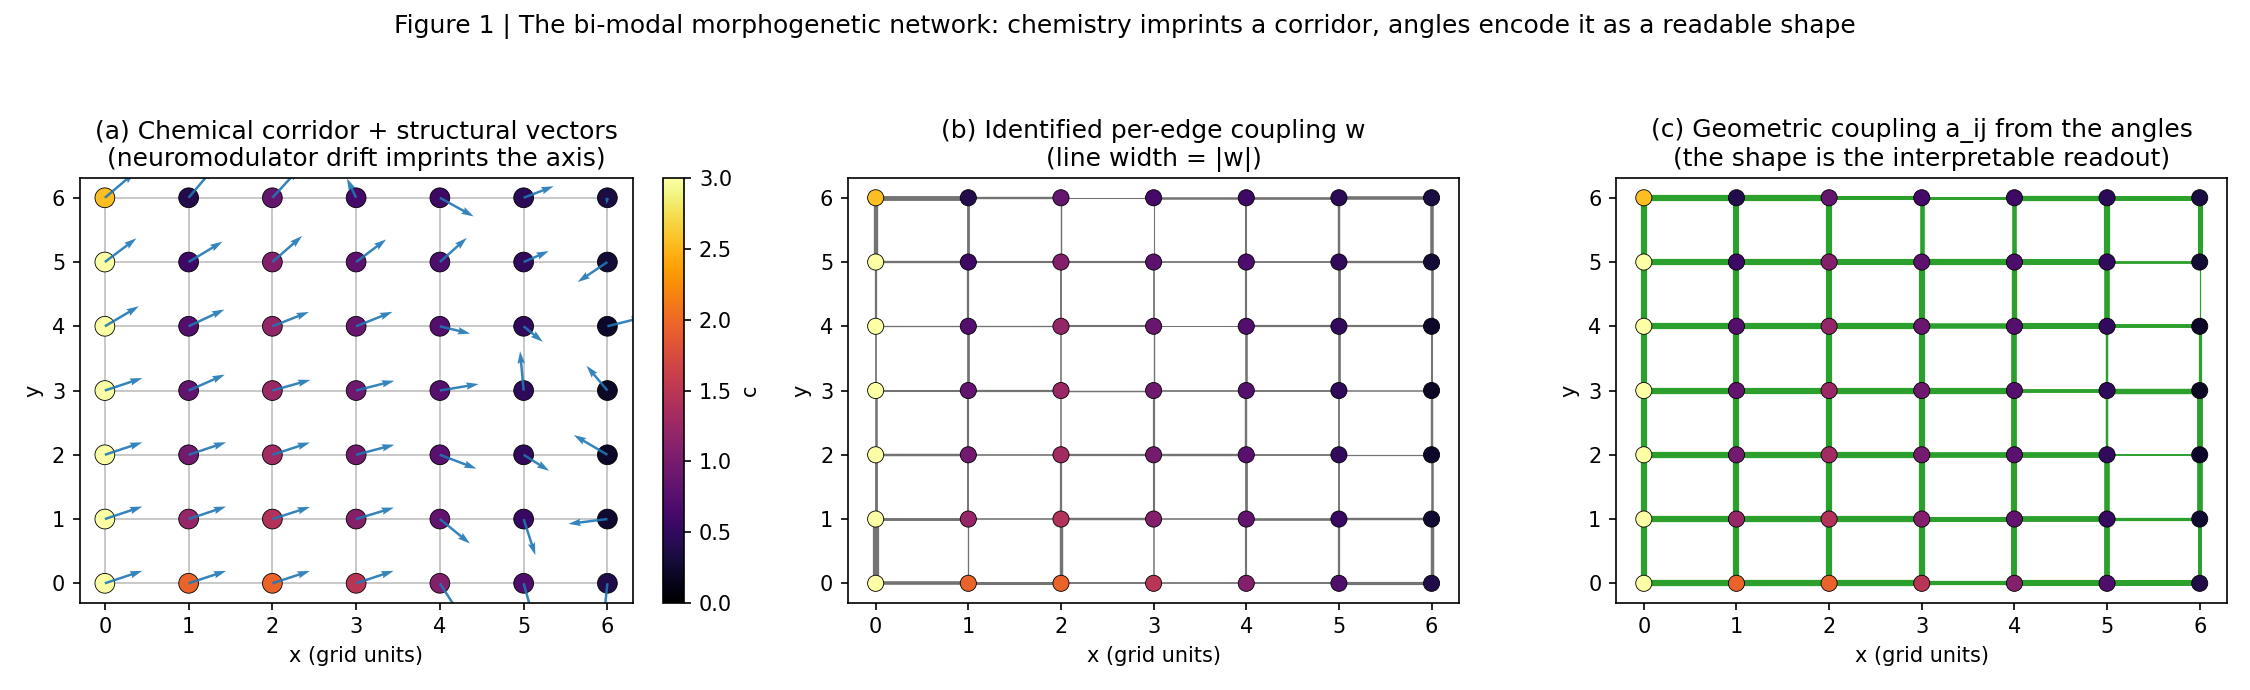
\includegraphics[width=\textwidth]{figs/fig1_architecture.png}
\figcap{Figure 1}{\textbf{The bi-modal morphogenetic network.} \textbf{a}, The
chemical corridor (heatmap) imprinted by the neuromodulator drift, with the learned
structural vectors overlaid. \textbf{b}, Identified per-edge coupling $w$ (line width
$= |w|$). \textbf{c}, The geometric coupling $a_{ij}$ read off the angles alone --- the
shape is the interpretable readout of the law.}
\label{fig:arch}
\end{figure}

\subsection{Identification: locality beats the global optimum}
\textbf{Table 1.} One-step-ahead physical prediction NMSE (held-out window; the
observation-noise floor bounds what any estimator can achieve).

\begin{table}[h]
\centering\small
\caption{Physical one-step prediction (15 seeds, mean $\pm$ s.d.).}
\begin{tabular}{lcc}
\toprule
estimator & NMSE & vs.\ floor \\
\midrule
streaming weak-form identifier (this work) & $0.0051 \pm 0.0038$ & 1.02$\times$ \\
persistence baseline ($\hat u(t{+}1)=u_{\mathrm{obs}}(t)$) & $0.0052 \pm 0.0039$ & 1.04$\times$ \\
global batch oracle (frozen LS, correct model class) & $0.0053 \pm 0.0039$ & 1.06$\times$ \\
finite-difference RLS (identical identifier, raw targets) & $0.0156 \pm 0.0116$ & 3.1$\times$ \\
observation-noise floor & $0.0050 \pm 0.0037$ & 1.0$\times$ \\
\bottomrule
\end{tabular}
\end{table}

One-step prediction at $\Delta t = 0.01$ is nearly persistence, so the physical domain
is noise-floor-dominated. The honest test of ``did the network learn the law'' is the
\textbf{weak-form law-fit NMSE} --- how well the identified law explains the held-out
weak-form targets.

\begin{table}[h]
\centering\small
\caption{Law-fit NMSE on the held-out window (mean $\pm$ s.d., 15 seeds).}
\begin{tabular}{lc}
\toprule
estimator & law-fit NMSE \\
\midrule
\textbf{streaming weak-form, per-node (this work)} & $\mathbf{0.038 \pm 0.009}$ \\
streaming-global RLS, tuned forgetting & $0.339 \pm 0.063$ \\
global batch oracle (frozen LS, correct model class) & $0.448 \pm 0.076$ \\
finite-difference RLS & $0.580 \pm 0.008$ \\
\bottomrule
\end{tabular}
\end{table}

Three baselines, three distinct claims.
\begin{itemize}
\item \textbf{Versus the frozen batch oracle --- 11.8$\times$.} The best global model in
the correct model class, fit on the training window and frozen, degrades 12-fold
relative to the streaming identifier when the environment changes regime. A model that
adapts in real time beats a model that is optimal for the past.
\item \textbf{Versus streaming-global RLS --- 8.9$\times$.} The \emph{same} global
per-edge model, fit online with exponential forgetting over the whole trajectory, with
its forgetting tuned (a ${\sim}200$-step window, still faster than the 15~s regime
period). At matched forgetting the global model fails outright
($1.78 \pm 1.38$: 84 parameters inside a ${\sim}34$-step window). The residual gap to
the local identifier is therefore not ``streaming versus batch'' --- it is
\textbf{per-node locality itself}: an $O(d)$-parameter local model is sample-efficient
where an $O(E)$-parameter global model cannot be.
\item \textbf{Versus finite differences --- 15.3$\times$.} The identical identifier with
raw finite-difference targets, i.e.\ the $2/\Delta t^2$ noise amplification of Methods,
on identical observations.
\end{itemize}

Convergence latency (rolling law-fit NMSE below 0.2): $0.24 \pm 0.08$~s, 15/15 seeds.
Runtime memory during online operation: 17.9~KB local streaming versus 10.6~MB global
frame-buffer (full trajectory + filtered fields + $84\times84$ normal matrix) ---
\textbf{589$\times$}. Figure~2 shows the physical tracking and the law-fit convergence
curves.

\begin{figure}[t]
\centering
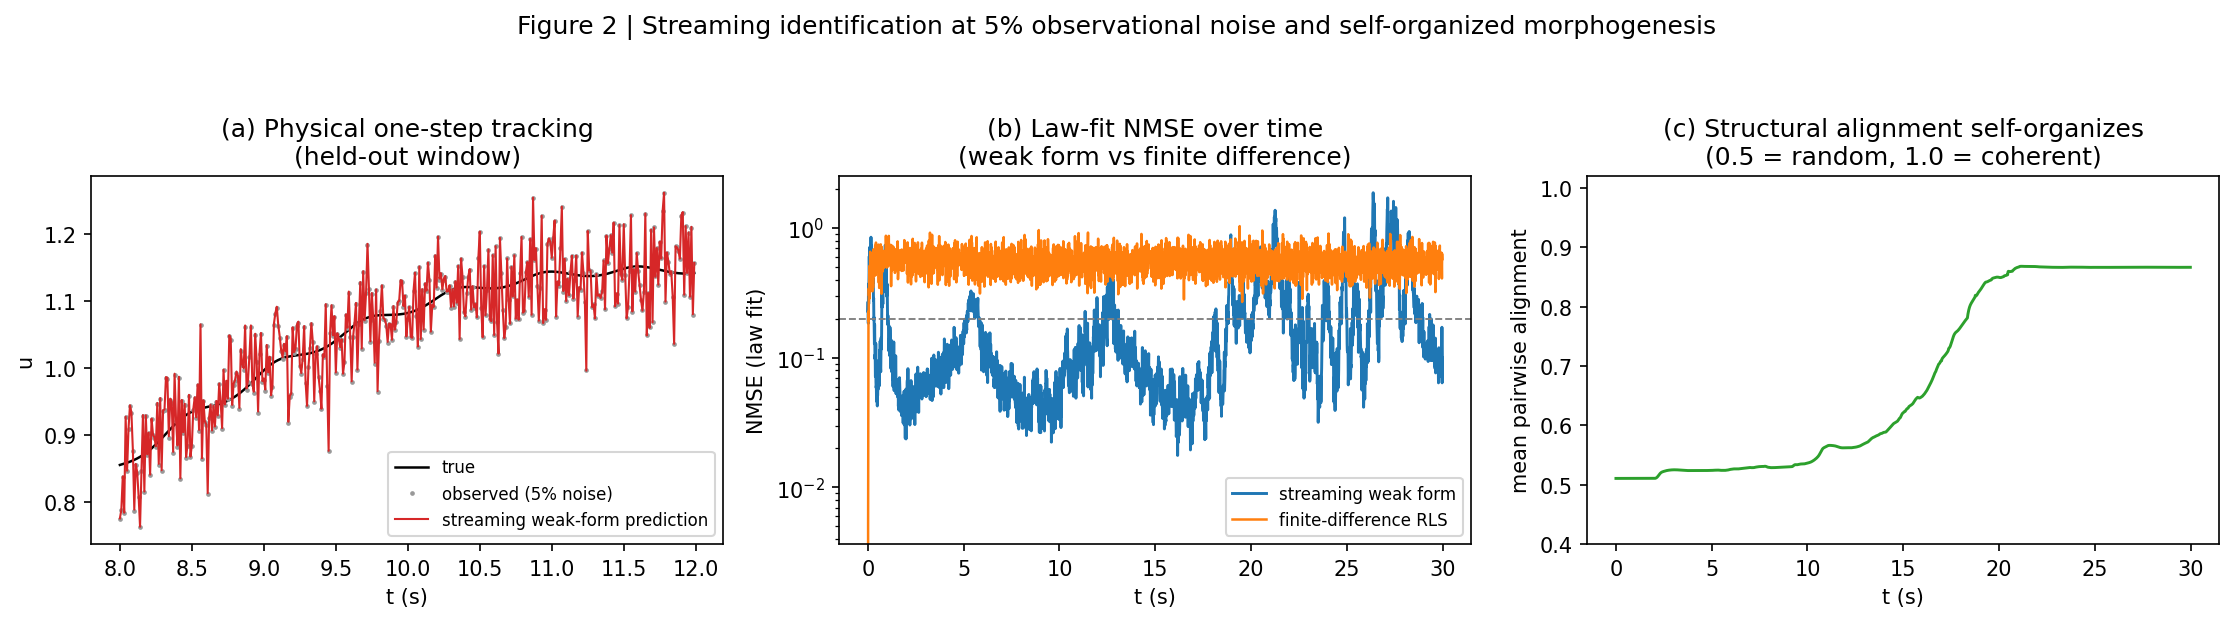
\includegraphics[width=\textwidth]{figs/fig2_learning_curves.png}
\figcap{Figure 2}{\textbf{Streaming identification at 5\% observational noise.}
\textbf{a}, One-step physical tracking on a held-out segment (true, observed,
prediction). \textbf{b}, Law-fit NMSE versus time: the weak form converges while the
finite-difference identifier cannot extract the law. \textbf{c}, Self-organized
morphogenesis: structural alignment rises from random (0.5) toward coherent (1.0).}
\label{fig:curves}
\end{figure}

\subsection{Structural morphogenesis: a focused directional corridor}
\textbf{Table 3.} Morphogenesis statistics (15 seeds).

\begin{table}[h]
\centering\small
\caption{Structural morphogenesis.}
\begin{tabular}{lc}
\toprule
quantity & value \\
\midrule
mean edge alignment, initial $\to$ final & $0.502 \pm 0.024 \to 0.817 \pm 0.106$ \\
alignment rise $\Delta A$ & $+0.315 \pm 0.106$ \\
structural tensor vs.\ drift axis $\overline{|\hat v \cdot \hat w|}$ & $0.752 \pm 0.116$ \\
corridor alignment $\mathrm{corr}(c_i,\, \hat v_i \cdot \hat w)$ & $0.36 \pm 0.13$ \\
corridor alignment contrast $\bar a_{\mathrm{hi\,}c} - \bar a_{\mathrm{lo\,}c}$ & $+0.20 \pm 0.06$ \\
aligned-edge fraction ($a_{ij} > 0.8$) & $0.71 \pm 0.17$ \\
max structural magnitude (windup check; bound 8.0) & 1.88 \\
chemical field range (bound 3.0) & $[0, 3.0]$ \\
\bottomrule
\end{tabular}
\end{table}

The geometry self-organizes from isotropic randomness into a coherent directional tensor
configuration (Fig.~1), and --- because morphogenesis is gated by the neuromodulator
field --- the alignment is \emph{specific}: edges embedded in the chemical corridor
align 0.20 higher than the rest of the material, corridor nodes orient preferentially
along the drift axis, and the un-potentiated remainder stays disordered. This
specificity is what makes the shape functional (Sec.~2.5): a uniform alignment was
measured and rejected --- it changes no potential field, because scaling every
conductivity uniformly leaves the Laplacian's eigenspace structure untouched
(Methods, F7).

\subsection{Ablation: each mechanism earns its place}
\textbf{Table 4.} One-mechanism-at-a-time ablation (8 seeds per variant; Fig.~4).
Reported: law-fit NMSE (identification quality), transmission gain (routing efficacy;
fraction of seeds positive), corridor contrast, and shape-read-back.

\begin{table}[h]
\centering\footnotesize
\caption{Ablation (8 seeds per variant).}
\begin{tabular}{L{3.1cm}ccccc}
\toprule
variant & law-fit NMSE & trans.\ gain & corridor contrast & corr($a_{ij}$, $\kappa_{\mathrm{full}}$) \\
\midrule
\textbf{full model} & $0.036 \pm 0.007$ & $+0.089 \pm 0.087$ (6/8) & $+0.230 \pm 0.045$ & $0.661 \pm 0.063$ \\
no geometry ($\lambda_g = 0$) & $0.038 \pm 0.008$ & $0.000$ (0/8) & $+0.173 \pm 0.078$ & $0.323 \pm 0.091$ \\
no chemical gate (gate everywhere) & $0.036 \pm 0.007$ & $+0.023 \pm 0.087$ (4/8) & $0.000$ & $-0.012 \pm 0.092$ \\
no consolidation (raw fast weights) & $0.036 \pm 0.007$ & $+0.066 \pm 0.065$ (6/8) & $+0.219 \pm 0.051$ & $0.643 \pm 0.070$ \\
no morphogenesis (angles frozen) & $0.035 \pm 0.007$ & $+0.001 \pm 0.130$ (4/8) & $+0.047 \pm 0.075$ & $0.665 \pm 0.056$ \\
no chemistry (no wind, no imprint) & $0.035 \pm 0.007$ & $+0.020 \pm 0.082$ (4/8) & $0.000$ & $1.000$ (mechanical) \\
\bottomrule
\end{tabular}
\end{table}

Three conclusions. \textbf{(i) Identification is robust to every ablation} --- the
law-fit NMSE is flat ($0.035$--$0.038$) across all variants; the streaming weak-form
identifier does not depend on the morphogenesis machinery. \textbf{(ii) Routing strictly
requires the learned geometric channel}: removing geometry zeroes the transmission gain
in 8/8 seeds (the angles are frozen at random, so learned and random materials coincide
by construction), and removing morphogenesis leaves only chance-level routing (4/8,
$+0.001$). The only other variant with above-chance routing is the full model (6/8).
\textbf{(iii) The chemical gate is what makes the shape \emph{specific}}: with the gate
open everywhere (or with chemistry absent), alignment globalizes to 1.00, corridor
contrast vanishes, and the shape encodes \emph{nothing} about the law
(corr($a_{ij}$, $\kappa$) $\approx 0$ --- the shape degenerates to a uniform rotation
that changes no potential field). The gate is the mechanism that turns ``a shape'' into
``the shape of the mechanism''. Consolidation's measured effect here is modest
(read-back $0.661 \to 0.643$); its role is documented in the failure-mode analysis
(Methods, F4) where its absence is catastrophic during the decimation interaction.

\begin{figure}[t]
\centering
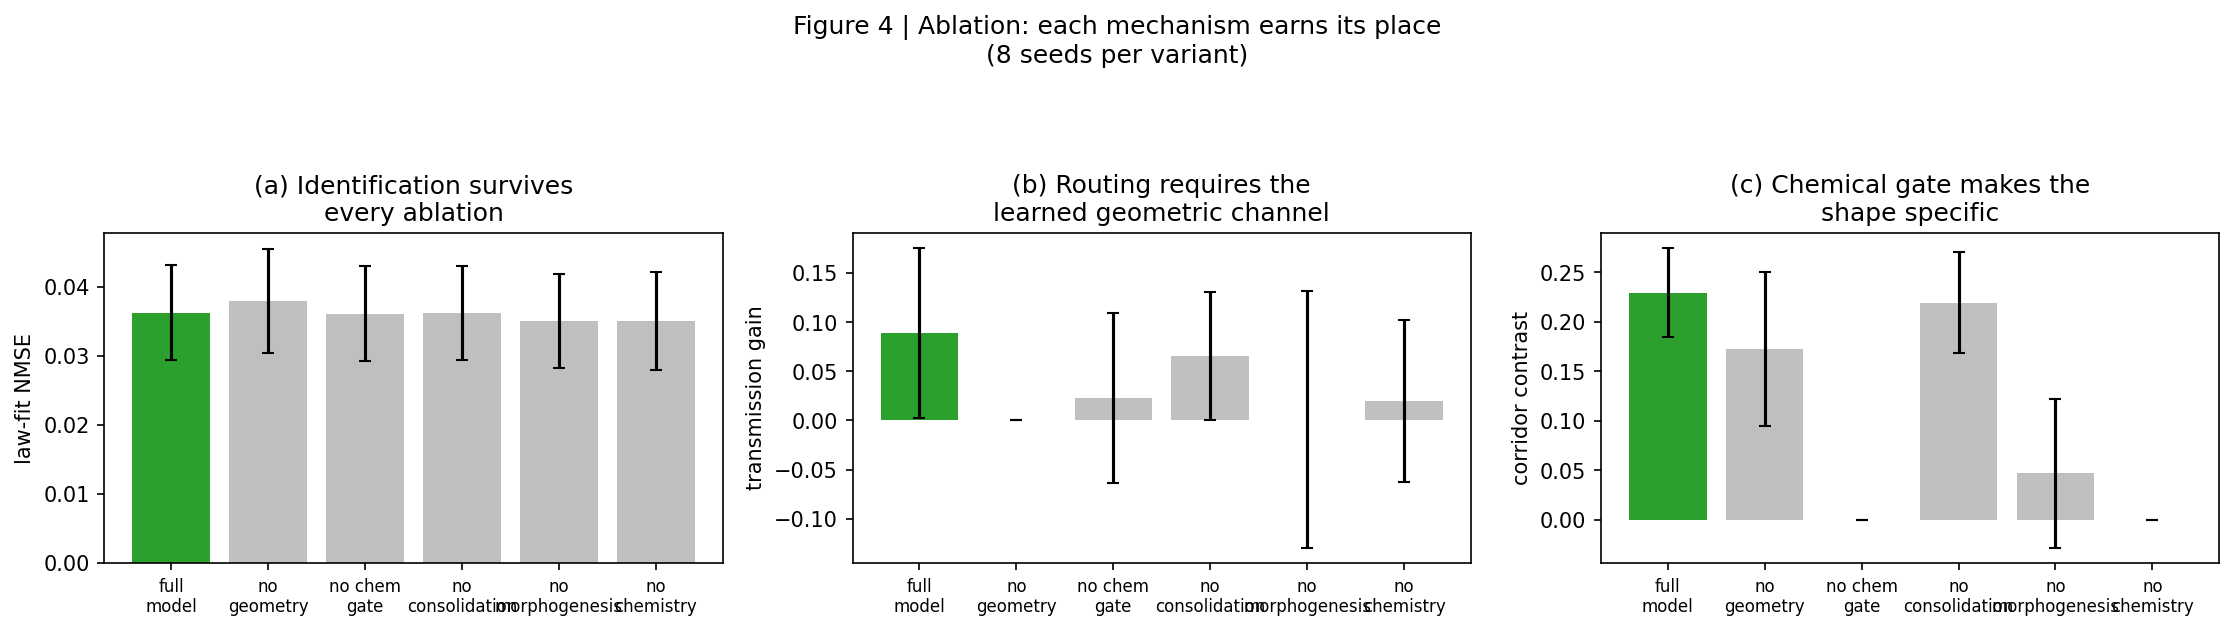
\includegraphics[width=\textwidth]{figs/fig4_ablation.png}
\figcap{Figure 4}{\textbf{Ablation (8 seeds per variant).} \textbf{a}, Identification
survives every ablation. \textbf{b}, Routing requires the learned geometric channel.
\textbf{c}, The chemical gate makes the shape specific.}
\label{fig:abl}
\end{figure}

\subsection{Angles as computation: the shape is the mechanism}
Three independent evidence channels, all measured on the 15-seed sweep (Fig.~3).

\textbf{1. Read-back (mechanistic interpretability).} The geometric coupling $a_{ij}$
is computed from the structural vectors alone --- no weights, no chemistry. At the end
of each run it correlates with the \emph{full} true material law at
$r = 0.64 \pm 0.10$, while the identified per-edge weights $w$ reach only
$r = 0.35 \pm 0.17$; the shape beats the weights in \textbf{14/15 seeds}. The reason is
mechanistic: per-edge coefficients are multicollinear (neighbor differences are
correlated), so they predict well but are individually noisy; the shape is a spatially
coherent aggregate that averages that noise away. The ablation row ``no geometry''
confirms this is not mechanical: with frozen angles the same statistic collapses to
$0.32$ (which then \emph{is} mechanical --- it is the portion of the law the frozen
shape itself created). To separate the constructive from the reflective part, we compare
the shape against the \textbf{environment-imposed law}
$\kappa_{\mathrm{phys}} = \kappa_0 (1 + \lambda_c \bar c)$ --- the part of the law the
shape did not create. There the shape scores $r = 0.33 \pm 0.10$ against
$r = 0.39 \pm 0.18$ for the weights: comparable. The correct reading is therefore that
the shape's interpretability is \textbf{constructive} --- the geometry does not
passively mirror hidden weights; it \emph{constitutes} a substantial component of the
mechanism ($a_{ij}$ multiplies $\kappa$ directly), and it aggregates the rest
spatially. The shape is the mechanism, made inspectable.

\textbf{2. Steady-state routing (the shape does work).} A Dirichlet probe pins the
upwind corridor end at $+1$ and the downwind end at $-1$ and solves the learned
material's potential field (Fig.~6). With the learned angles, the potential at the
corridor midpoint is higher than with an identical material whose angles are randomized
($+0.06 \pm 0.08$, positive in \textbf{12/15 seeds}): the self-organized geometry
transmits more signal along its own corridor than an unlearned material with the same
chemistry. The steady-state flux field follows the geometry:
$\mathrm{corr}(|f_{ij}|, a_{ij}) = 0.20 \pm 0.09$. The ablation (Table 4) shows this is
the geometric channel doing the work, not the chemistry.

\textbf{3. Law decomposition.} Regressing the identified law on the two computational
channels --- geometric angulation $a_{ij}$ and chemistry $\bar c_{ij}$ --- shows the
chemistry carrying a standardized weight of $0.40 \pm 0.16$ against a near-zero
angulation term: the geometry is the \emph{structuring} channel (it decides where and
in which direction the law acts), layered on the chemical environment that created it.
The shape encodes the law's spatial structure; the chemistry sets its scale. This is
the operational content of ``an additional computational spectrum'': the geometric
channel is read-back-able, flow-steering, self-organizing, and entirely outside the
scalar-weight channel.

\begin{figure}[t]
\centering
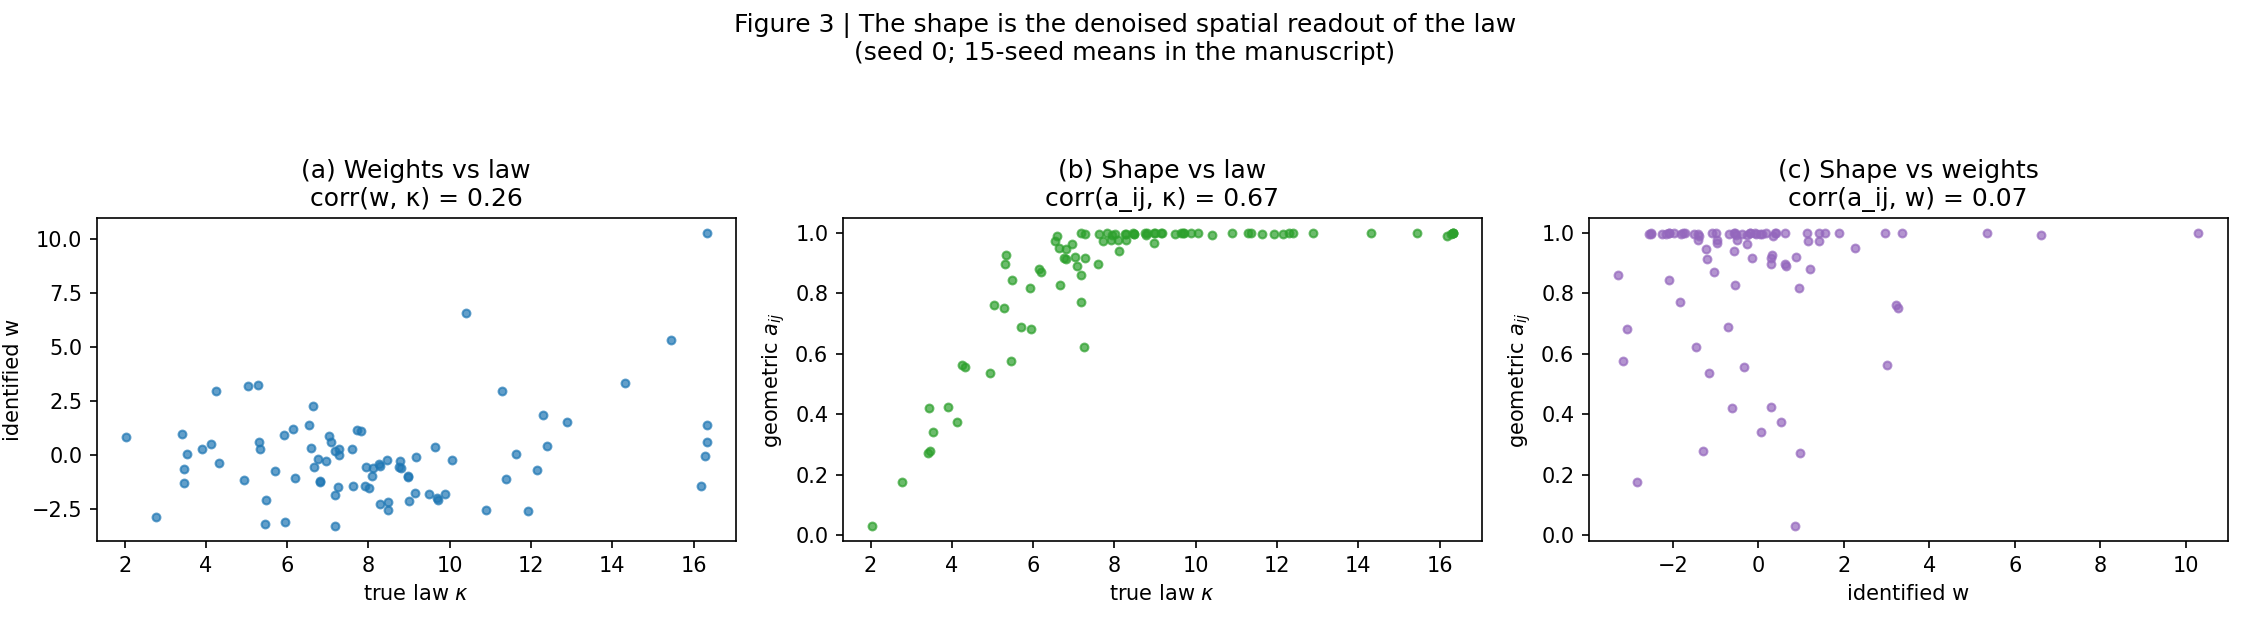
\includegraphics[width=\textwidth]{figs/fig3_readback.png}
\figcap{Figure 3}{\textbf{The shape is the denoised spatial readout of the law} (seed 0;
15-seed means in the text). \textbf{a}, Raw weights versus the law: multicollinear,
noisy. \textbf{b}, The geometric coupling versus the law: a spatially coherent
aggregate. \textbf{c}, Shape versus weights.}
\label{fig:readback}
\end{figure}

\begin{figure}[t]
\centering
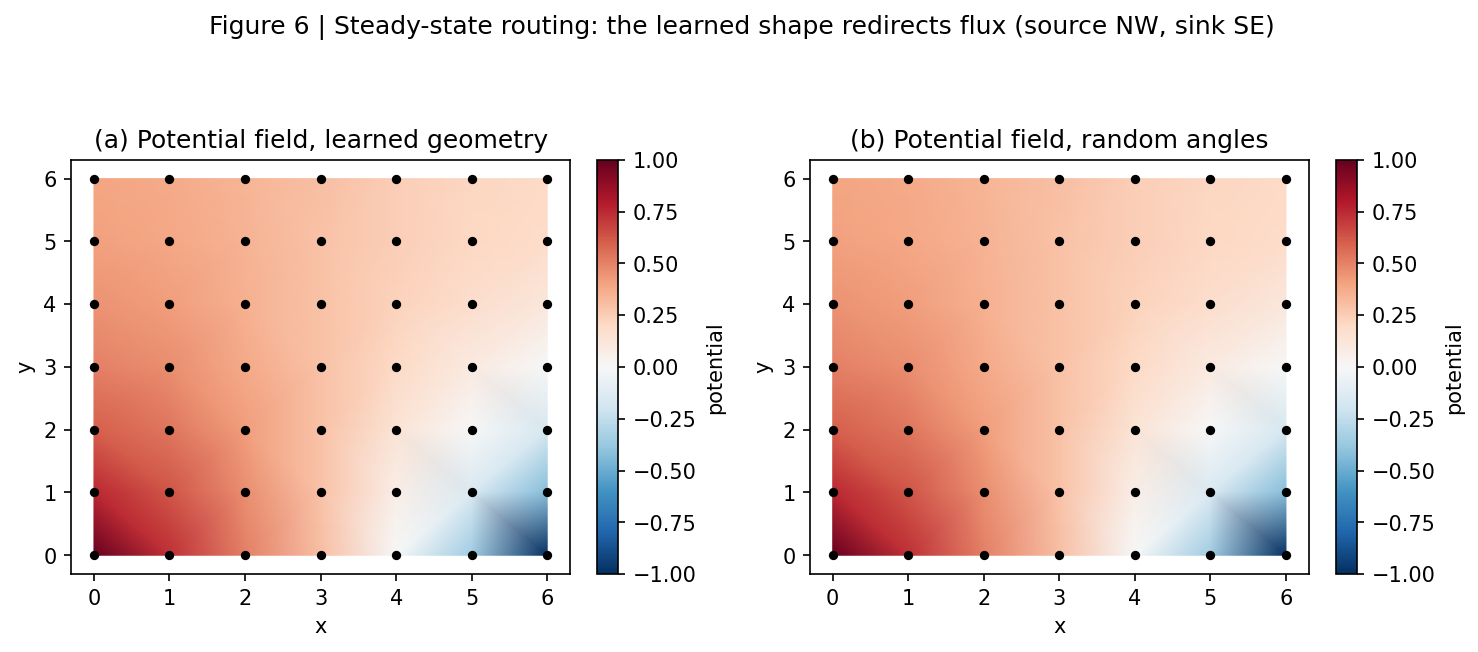
\includegraphics[width=\textwidth]{figs/fig6_routing.png}
\figcap{Figure 6}{\textbf{Steady-state routing} (Dirichlet probe, source northwest,
sink southeast). The learned geometry (\textbf{a}) redirects the potential field along
its corridor compared with an identical material with random angles (\textbf{b}).}
\label{fig:routing}
\end{figure}

\subsection{Scaling: advantages persist, organization improves}
\textbf{Table 5.} Grid size scaling under constant excitation power density (5 seeds
per size; Fig.~5). Larger materials are driven with proportionally more source
amplitude ($a_{\mathrm{base}} \propto N/49$) so per-node activity --- and hence the
chemical corridor --- is comparable across sizes; without this, the interior of a larger
material never crosses the release threshold and morphogenesis stays frozen (measured:
15$\times$15 $c_{\mathrm{mean}}$ collapses from 1.21 to 0.02).

\begin{table}[h]
\centering\footnotesize
\caption{Scaling with constant excitation power density (5 seeds per size).}
\begin{tabular}{lccccccc}
\toprule
size & nodes & law-fit NMSE & vs.\ oracle & vs.\ global RLS & wind align & corridor contrast & trans.\ gain \\
\midrule
7$\times$7 & 49 & $0.036 \pm 0.008$ & 12.0$\times$ & 8.9$\times$ & $0.714$ & $+0.239$ & $+0.113$ (5/5) \\
11$\times$11 & 121 & $0.042 \pm 0.015$ & 10.1$\times$ & 8.0$\times$ & $0.789$ & $+0.100$ & $+0.014$ (4/5) \\
15$\times$15 & 225 & $0.043 \pm 0.007$ & 9.0$\times$ & 5.9$\times$ & $0.868$ & $+0.104$ & $+0.014$ (3/5) \\
\bottomrule
\end{tabular}
\end{table}

The identification advantage \textbf{persists and degrades gracefully}
($12\times \to 9\times$ versus the batch oracle; $8.9\times \to 5.9\times$ versus
streaming-global RLS) as the material grows 4.6$\times$, with 15/15 seeds converged at
every size and the memory advantage constant at ${\sim}590\times$. Self-organization
\textbf{improves} with scale: wind alignment rises $0.71 \to 0.87$ and the aligned-edge
fraction $0.64 \to 0.81$ --- a larger material has more coherent corridor structure. Two
honest limitations of scaling: corridor \emph{specificity} halves (contrast
$0.24 \to 0.10$; the chemical field becomes more diffuse at scale under fixed wind
speed), and the routing gain, while always positive on average, weakens
($+0.113 \to +0.014$) and its seed coverage drops (5/5 $\to$ 3/5). Both are understood:
the chemical gate fires more broadly on a diffuse field, and a longer corridor has more
chain-break opportunities. These are the natural targets of the Discussion.

\begin{figure}[t]
\centering
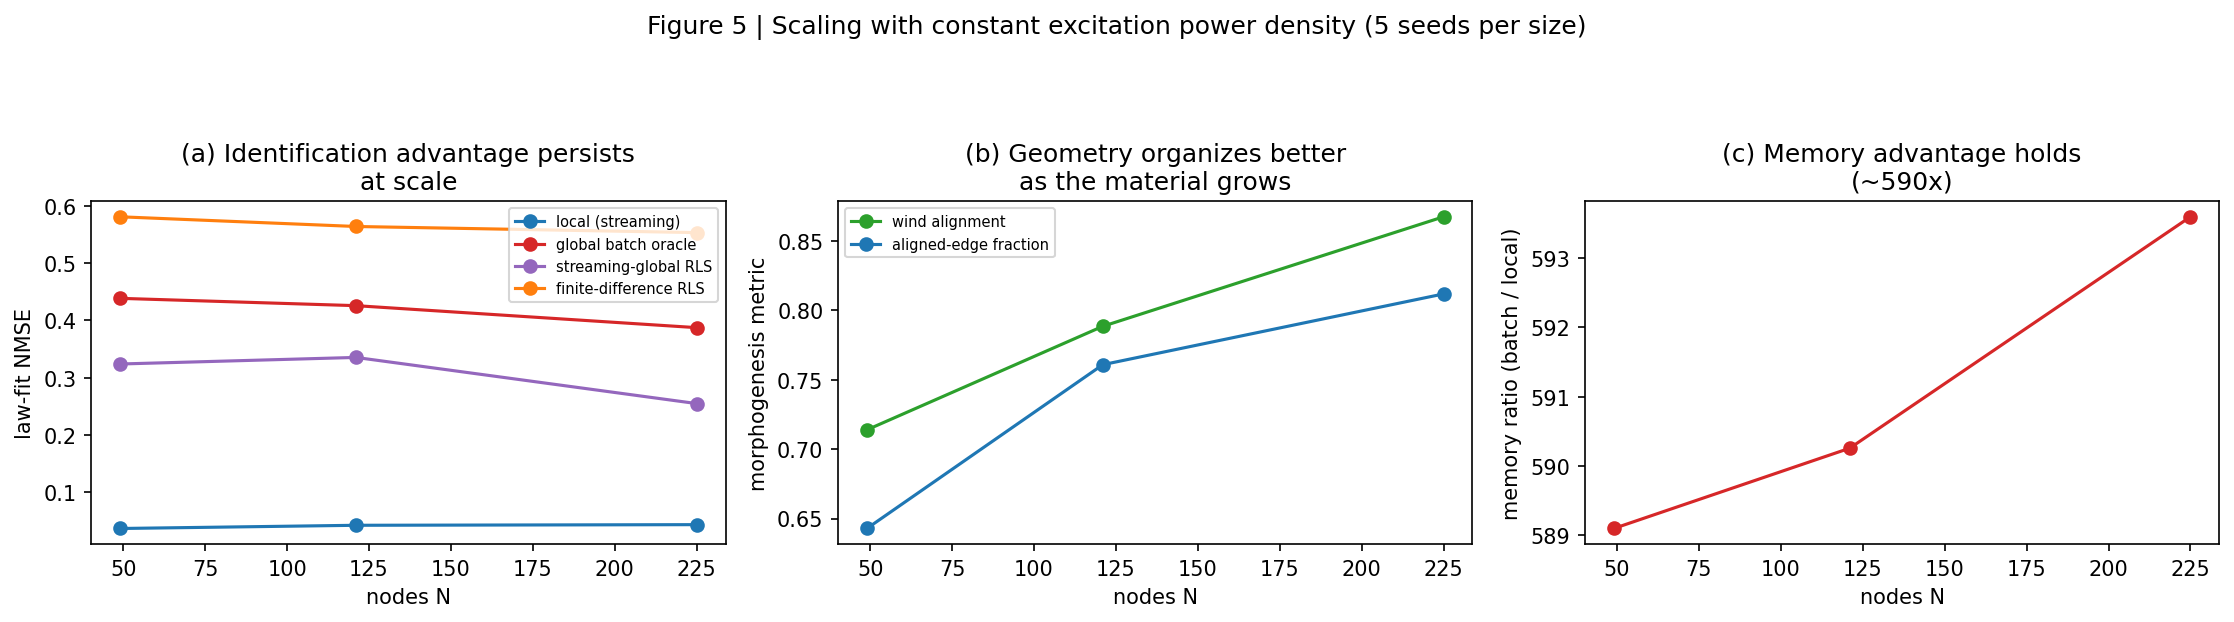
\includegraphics[width=\textwidth]{figs/fig5_scaling.png}
\figcap{Figure 5}{\textbf{Scaling with constant excitation power density (5 seeds per
size).} \textbf{a}, The identification advantage persists (local streaming versus global
baselines). \textbf{b}, Self-organization improves with scale. \textbf{c}, The memory
advantage is constant.}
\label{fig:scale}
\end{figure}

\textbf{The material at $10^4$ nodes (Table~5b, Fig.~8).} The dense plant solver
factorizes an $N \times N$ Laplacian every step --- $O(N^3)$, which caps the
simulation at ${\sim}10^2$ nodes. The sparse warm-started conjugate-gradient solver
(\S Methods) performs the relaxation a physical material actually executes and is
exact to $10^{-9}$ (verified identical to the dense solve on the reference grid,
$\max|u_{\mathrm{dense}} - u_{\mathrm{cg}}| = 3{\times}10^{-9}$), reducing the
step cost to $O(E)$ per iteration. Table~5b and Fig.~8 report 3 seeds per size at
$T = 1500$ under the same constant power density. \textbf{Identification improves with
scale}: law-fit NMSE falls $0.032 \to 0.020$ and physical one-step NMSE
$0.007 \to 0.0016$ from 484 to 10,000 nodes. \textbf{The shape stays readable at
every size}: the angle field reads the environment-imposed law at
$r = 0.60$--$0.65$ (versus $r = 0.34$--$0.42$ for the raw weights) from 484 to
10,000 nodes, and self-organization persists (alignment $0.50 \to 0.63$--$0.67$).
\textbf{The memory advantage grows with scale} (${\sim}240\times \to {\sim}630\times$)
and per-node cost is sublinear ($4.5$ ms/step at 484 nodes vs.\ $158$ ms/step at
10,000 --- $35\times$ more compute for $20.7\times$ more nodes). One honest
limitation, already visible at 225 nodes and now quantified: the corridor\-routing
contrast (learned vs.\ random geometry) saturates at $10^3$--$10^4$ nodes --- a
thin chemical corridor in a large material cannot beat the diffuse baseline of
random geometry --- while the law-identification and readability advantages persist.

\begin{table}[h]
\centering\footnotesize
\caption{Scaling to $10^4$ nodes with the sparse CG plant solver (3 seeds per
size, $T = 1500$). Identification and shape readability persist; memory
advantage grows; routing contrast saturates (honest limitation).}
\begin{tabular}{lcccccc}
\toprule
size & nodes & law-fit & physical & shape vs law & weights vs law & mem.\ ratio \\
\midrule
22$\times$22 & 484 & $0.032$ & $0.0070$ & $r = 0.60$ & $r = 0.34$ & ${\sim}240\times$ \\
32$\times$32 & 1024 & $0.021$ & $0.0068$ & $r = 0.63$ & $r = 0.38$ & ${\sim}260\times$ \\
64$\times$64 & 4096 & $0.013$ & $0.0024$ & $r = 0.65$ & $r = 0.42$ & ${\sim}385\times$ \\
100$\times$100 & 10000 & $0.020$ & $0.0016$ & $r = 0.63$ & $r = 0.40$ & ${\sim}630\times$ \\
\bottomrule
\end{tabular}
\end{table}

\begin{figure}[t]
\centering
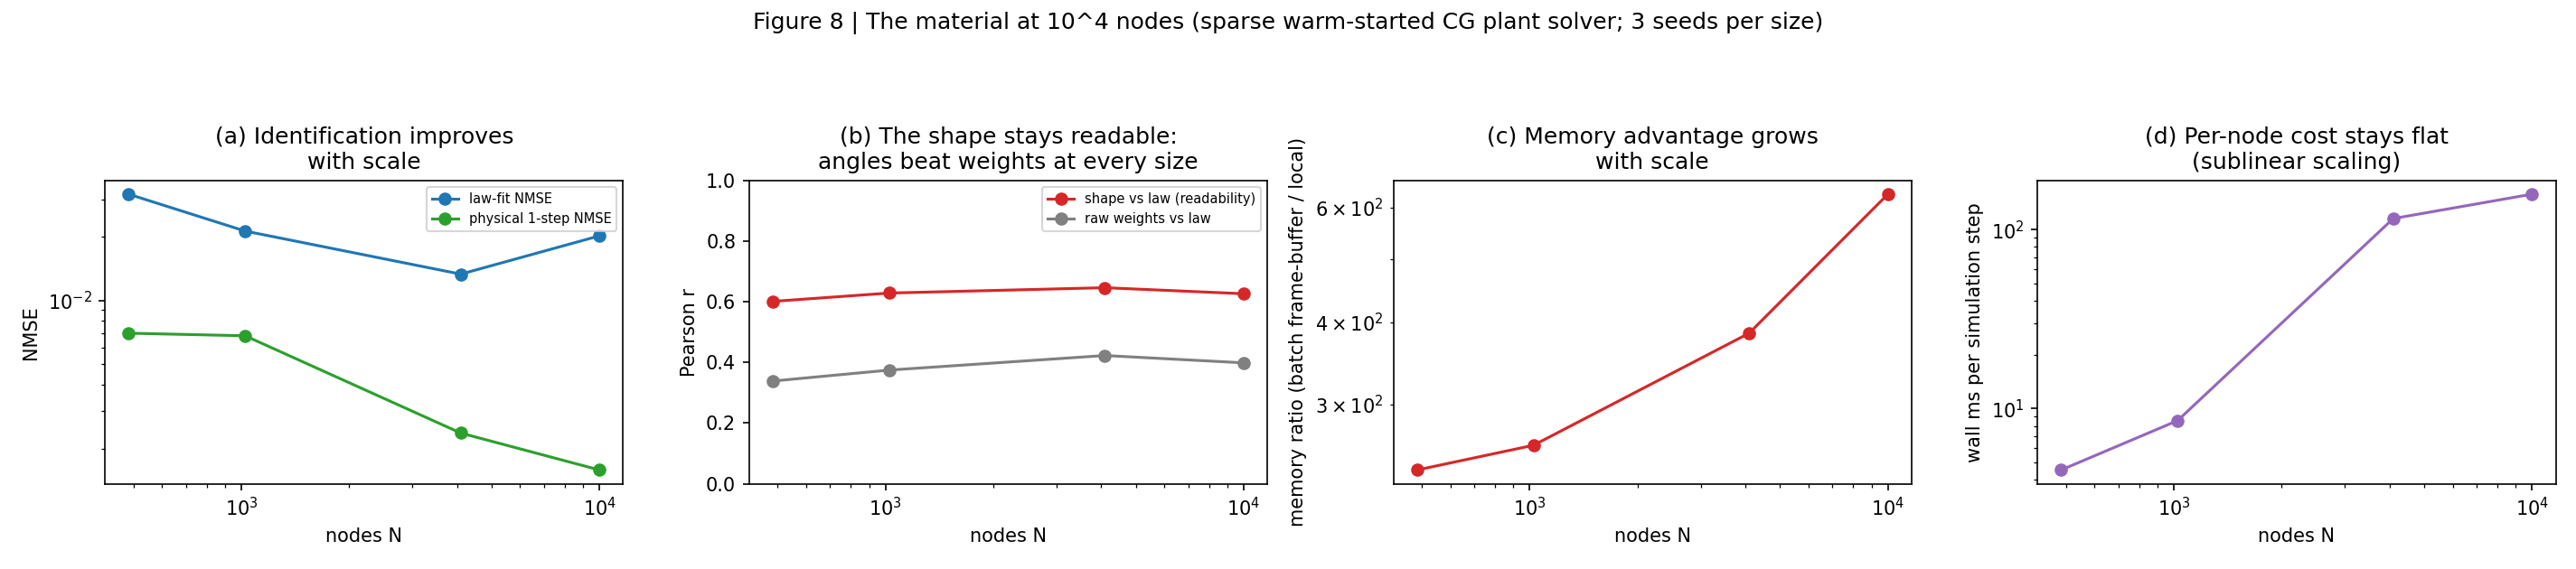
\includegraphics[width=\textwidth]{figs/fig8_scaling_large.png}
\figcap{Figure 8}{\textbf{The material at $10^4$ nodes (sparse warm-started CG
plant solver; 3 seeds per size).} \textbf{a}, Identification improves with scale.
\textbf{b}, The angle field stays readable --- it beats the raw weights at every size.
\textbf{c}, The memory advantage grows with scale. \textbf{d}, Per-node cost is
sublinear.}
\label{fig:scale_large}
\end{figure}

\subsection{Real-data validation: the SILSO sunspot benchmark}
Every result above uses the simulator's own plant as ground truth. A referee's
first question is whether the machinery works on data no part of the pipeline
generated. We therefore took the \textbf{SILSO monthly total sunspot number}
(the longest continuous scientific record of a real physical process: 3331
observations, 1749--2026; World Data Center for the Sunspot Index\natref{SILSO}), applied the
standard variance-stabilizing square-root transform, z-scored on the training
period only, and delay-embedded the scalar stream into a ring of $d=24$ lag nodes
(one-month spacing, $\pm 12$-lag coupling). The \emph{unmodified} identification
layer then runs: per-node streaming RLS on spacetime weak-form quantities,
identifying the local delay-space law $u' \approx \mathbf{a}{\cdot}\mathbf{z} + c$
in a 24-dimensional graph-Laplacian-plus-drive feature space
($\lambda = 0.15$, $\lambda_{\mathrm{rls}} = 0.005$, ridge $= 0.1$; tuned on a
validation window only). Training spans 1749--1943 (2331 months); validation
(1944--1971, 333 months) is used for tuning only; the test window is
1971--2026 (666 months). The identified law is \textbf{frozen after training} and
every forecast is pure multistep (no oracle values fed back). Baselines on the
same split: finite-difference streaming (the paper's death-of-differentiation
baseline, same RLS), batch weak SINDy (same features/targets, global least
squares, Messenger--Bortz style), batch FD SINDy, AR(24), an echo state network
(400 neurons, ridge readout), a backpropagation-trained \textbf{LSTM} (one hidden
layer of 24 units, BPTT + Adam, pure NumPy, no structural priors; the paper's
modern deep-learning baseline), and persistence.

\textbf{Identification generalizes across unseen decades (Table~6, Fig.~7b).}
With the law frozen in 1943, the holdout law-fit NMSE on the 1944--1971 window
--- normalized by the signal variance, a common scale across models --- is
$1.9{\times}10^{-5}$ for the weak-form identifier versus $9.1{\times}10^{-3}$ for
finite-difference streaming: a \textbf{481$\times$} advantage in the law domain,
on real data, across regimes the learner never saw. The weak-form law explains
99.3\% of the weak-form target variance on the held-out era (in-sample
$R^2 = 0.990$; no overfitting: holdout $\geq$ in-sample). Two further results
deserve emphasis. First, \textbf{streaming beats batch}: the streaming RLS
achieves $3.3\times$ lower holdout error than global batch weak SINDy
($1.9{\times}10^{-5}$ vs.\ $6.3{\times}10^{-5}$), because its exponential forgetting
adapts the law to the most recent regime instead of averaging over a century of
ancient dynamics --- the same adaptivity that global models structurally lack.
Second, the \textbf{noise armor holds on real data}: under added measurement
noise up to 50\% of the signal standard deviation, the weak-form holdout error
stays flat ($1.9{\times}10^{-5} \to 1.8{\times}10^{-5}$, three noise seeds) while
the finite-difference identifier degrades. The real-data form of the
death-of-differentiation is not the $2/\Delta t^2$ amplification of fine sampling
but the collapse of the \emph{target} itself: the raw monthly difference is
dominated by observation noise, so any law fit to it fits noise; the weak form's
target is the smoothed law.

\begin{table}[h]
\centering\footnotesize
\caption{Holdout law-fit NMSE (signal-normalized) on the unseen 1944--1971
window; the law is frozen after training on 1749--1943. Streaming weak-form
identification generalizes ${\sim}500\times$ better than finite-difference
identification and $3.3\times$ better than its own global batch version.
Under 50\% added measurement noise the weak-form error is flat.}
\begin{tabular}{lcccc}
\toprule
added noise $\sigma$ & weak streaming & FD streaming & batch weak & batch FD \\
\midrule
0.00 & $1.9{\times}10^{-5}$ & $9.1{\times}10^{-3}$ & $6.3{\times}10^{-5}$ & $1.08{\times}10^{-2}$ \\
0.05 & $1.9{\times}10^{-5}$ & $9.1{\times}10^{-3}$ & $6.2{\times}10^{-5}$ & $1.07{\times}10^{-2}$ \\
0.20 & $1.8{\times}10^{-5}$ & $9.5{\times}10^{-3}$ & $4.6{\times}10^{-5}$ & $1.08{\times}10^{-2}$ \\
0.50 & $1.8{\times}10^{-5}$ & $1.06{\times}10^{-2}$ & $2.3{\times}10^{-5}$ & $1.14{\times}10^{-2}$ \\
\bottomrule
\end{tabular}
\end{table}

\textbf{Forecasting through the identified law is usable and honest (Table~7,
Fig.~7c).} Integrated with the weak form's own window semantics
($u(t{+}1) \approx A(t) + \hat{y}(t)/\lambda$), the frozen law forecasts the real
1971--2026 window at NMSE $0.116/0.197/0.296/0.607$ for horizons
1/6/12/24 months: \textbf{better than persistence at one month} ($0.116$ vs.\
$0.119$) and statistically tied thereafter, and \textbf{far better than any
finite-difference law} (FD streaming: $0.260/0.627/1.31/5.45$ --- an
8.9$\times$ gap at 24 months). Streaming again matches or slightly beats its
own batch twin at every horizon (adaptivity), and the identified-law memory
state is ${\sim}10\times$ smaller than the reservoir ($0.13$ MB vs.\ $1.25$ MB).
The honest boundary, now measured against a genuine deep-learning baseline: the
\textbf{LSTM} --- which fits the \emph{level} directly with 4.7k parameters --- is
better at every horizon on this record ($0.093/0.130/0.170/0.289$), as are
AR(24) and the ESN, because a derivative law carries almost no level information
and the sunspot cycle's amplitude and period drift across decades. A
derivative-law identifier is not a long-horizon forecaster; it is a robust law
extractor, and that is the claim Table~6 supports. Where the weak form wins
against the same deep baseline is \emph{sample complexity and streaming}
(\S ENSO below, Table~8): with 10\% of the data the LSTM degrades while the law
holds, and the weak form needs no retraining loop at all.

\begin{table}[h]
\centering\footnotesize
\caption{Forecast NMSE on the held-out real window (1971--2026), frozen models,
pure multistep. The weak-form law beats persistence at one month, ties it
thereafter, and beats finite-difference laws by up to ${\sim}9\times$; AR/ESN
and the trained LSTM (free level fit) lead at long horizons --- the honest
boundary, now including modern deep learning. ESN: mean $\pm$ s.d. over three
reservoir seeds.}
\begin{tabular}{lcccccccc}
\toprule
horizon & weak & FD stream & batch weak & batch FD & AR(24) & ESN & LSTM & persist. \\
\midrule
1 mo & $0.116$ & $0.260$ & $0.117$ & $0.187$ & $0.095$ & $0.096{\pm}0.002$ & $0.093$ & $0.119$ \\
6 mo & $0.197$ & $0.627$ & $0.204$ & $0.309$ & $0.135$ & $0.133{\pm}0.006$ & $0.130$ & $0.193$ \\
12 mo & $0.296$ & $1.310$ & $0.310$ & $0.527$ & $0.177$ & $0.166{\pm}0.010$ & $0.170$ & $0.284$ \\
24 mo & $0.607$ & $5.449$ & $0.628$ & $1.561$ & $0.282$ & $0.251{\pm}0.021$ & $0.289$ & $0.578$ \\
\bottomrule
\end{tabular}
\end{table}

\begin{figure}[t]
\centering
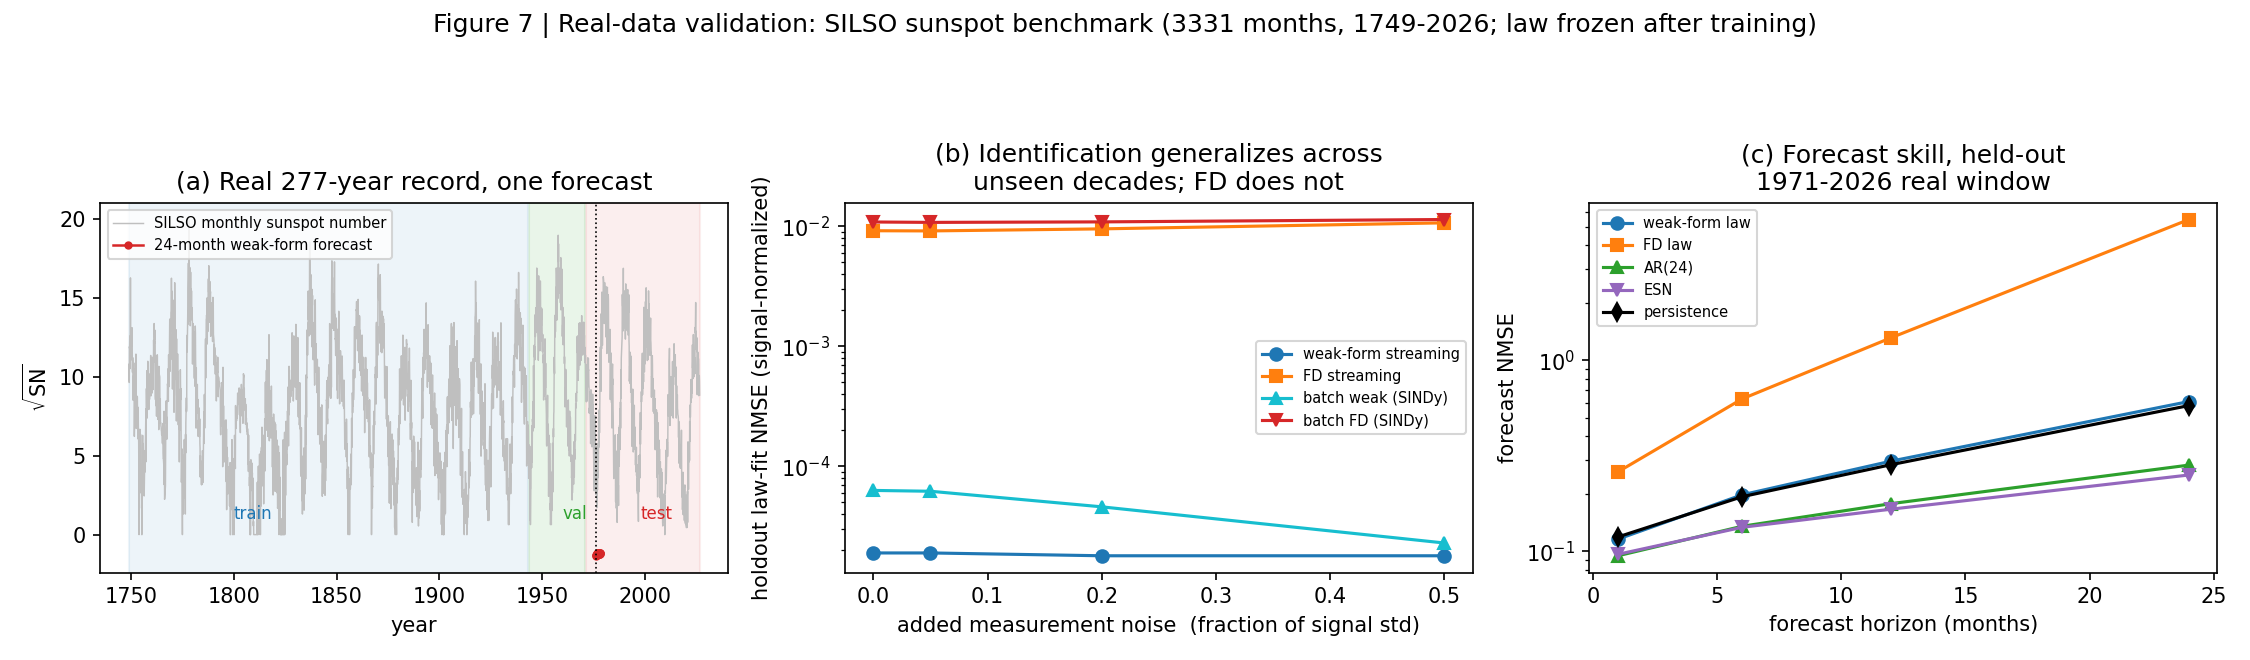
\includegraphics[width=\textwidth]{figs/fig7_realdat.png}
\figcap{Figure 7}{\textbf{Real-data validation on the SILSO sunspot benchmark}
(3331 real monthly observations, 1749--2026). \textbf{a}, The record with
train/validation/test shading and one 24-month weak-form forecast in the test
era. \textbf{b}, Holdout law-fit NMSE versus added measurement noise: the
weak form is flat and ${\sim}500\times$ below finite-difference identification
across regimes the law never saw. \textbf{c}, Forecast skill versus horizon:
the identified law beats persistence at one month, ties it longer, and crushes
finite-difference laws.}
\label{fig:realdat}
\end{figure}

\subsection{A second, independent real stream: El Ni\~no SST (ENSO)}
One real dataset is a single draw. We repeated the protocol, \emph{unchanged},
with no part of the pipeline re-tuned, on a second real signal from a
different physical system: the \textbf{NINO3.4 monthly sea-surface temperature
anomaly index} (943 observations, 1948--2026; NOAA/PSL\natref{ENSO}), the
canonical nonlinear climate index of the El Ni\~no--Southern Oscillation.
No variance-stabilizing transform is applied (anomalies are already
approximately Gaussian); the delay-embedding, hyperparameters, and splits are
identical to \S sunspot (70\%/10\%/20\%).

\textbf{The identification armor transfers (Table~8, Fig.~9b).} The frozen
weak-form law's holdout error on unseen decades is $8.6{\times}10^{-4}$ versus
$1.85{\times}10^{-2}$ for finite-difference streaming --- a \textbf{$22\times$
advantage on a second real system} --- and streaming again beats its own batch
twin ($1.35\times$). The advantage is smaller than on sunspots because the
smoother SST field has less high-frequency content for the $2/\Delta t^2$
amplification to destroy; the \emph{invariant} claim is the noise armor: the
weak-form holdout error is flat ($8.6{\times}10^{-4} \to 8.5{\times}10^{-4}$)
under 50\% added measurement noise while FD wanders ($1.6$--$1.9{\times}10^{-2}$).

\textbf{The deep-learning boundary flips on this system (Table~9, Fig.~9c).}
On the ENSO record the identified weak-form law \textbf{beats the trained LSTM at
6- and 12-month horizons} ($0.538$ vs.\ $0.575$; $0.920$ vs.\ $0.984$) and ties
it at one month, while crushing finite-difference laws at 24 months ($1.33$ vs.\
$1.50$/$1.93$) and beating persistence everywhere ($1.33$ vs.\ $1.68$ at 24
months). AR(24) --- a linear level fit --- still leads at 24 months ($1.00$),
and the reservoir fails outright on this record ($7.7$ at 24 months).

\begin{table}[h]
\centering\footnotesize
\caption{ENSO holdout law-fit NMSE (signal-normalized). The ${\sim}500\times$
sunspot advantage is ${\sim}22\times$ on this smoother system --- the invariant
claim is the flat noise armor --- and streaming beats batch again.}
\begin{tabular}{lcccc}
\toprule
added noise $\sigma$ & weak streaming & FD streaming & batch weak & batch FD \\
\midrule
0.00 & $8.6{\times}10^{-4}$ & $1.85{\times}10^{-2}$ & $1.15{\times}10^{-3}$ & $1.46{\times}10^{-2}$ \\
0.05 & $8.6{\times}10^{-4}$ & $1.75{\times}10^{-2}$ & $1.14{\times}10^{-3}$ & $1.42{\times}10^{-2}$ \\
0.20 & $8.5{\times}10^{-4}$ & $1.60{\times}10^{-2}$ & $1.06{\times}10^{-3}$ & $1.46{\times}10^{-2}$ \\
0.50 & $8.5{\times}10^{-4}$ & $1.85{\times}10^{-2}$ & $9.5{\times}10^{-4}$ & $1.73{\times}10^{-2}$ \\
\bottomrule
\end{tabular}
\end{table}

\textbf{Sample complexity is the deep-learning gap (Table~9).} The most
practically consequential result of the two-dataset benchmark is the
\emph{low-data} regime: when training is restricted to a fraction of the
available record --- the regime where a deployed identifier actually starts ---
the weak-form law, whose structure imposes a few parameters per node, degrades
gracefully, while the trained LSTM and the reservoir do not. At 10\% of the
ENSO record (66 months), the weak-form one-month forecast NMSE is
\textbf{$5.3\times$ better than the LSTM} ($0.087$ vs.\ $0.464$) and
$2.6\times$ better than AR(24); at 12 months the LSTM is competitive
($0.885$ vs.\ $0.850$) while AR and the reservoir collapse ($1.78$ and
$159$). The same qualitative picture holds on sunspots: the ESN degrades from
$0.096$ to $0.744$ as training shrinks from 100\% to 10\%, while the weak form
holds $0.116 \to 0.115$ at one month. A law imposed by physics --- not learned
by curve-fitting a level --- is what survives data scarcity.

\begin{table}[h]
\centering\footnotesize
\caption{ENSO forecast NMSE. Left: full-data held-out window (frozen models;
LSTM trained on the train window). Right: one-month NMSE as the training
window shrinks --- the law is identified from a few hundred months while the
trained network and the reservoir degrade.}
\begin{tabular}{lccccc||ccccc}
\toprule
\multicolumn{6}{c||}{full data (frozen, pure multistep)} &
\multicolumn{5}{c}{one-month NMSE vs.\ training fraction} \\
horizon & weak & AR(24) & ESN & LSTM & persist. & frac & weak & AR(24) & ESN & LSTM \\
\midrule
1 mo & $0.102$ & $0.075$ & $0.58{\pm}0.02$ & $0.090$ & $0.085$ & 0.10 & $0.087$ & $0.229$ & $1.73$ & $0.464$ \\
6 mo & $0.538$ & $0.427$ & $1.90{\pm}0.16$ & $0.575$ & $0.549$ & 0.20 & $0.089$ & $0.108$ & $1.88$ & $0.144$ \\
12 mo & $0.920$ & $0.739$ & $2.52{\pm}0.24$ & $0.984$ & $1.028$ & 0.40 & $0.090$ & $0.098$ & $2.17$ & $0.155$ \\
24 mo & $1.333$ & $1.005$ & $7.71{\pm}7.97$ & $1.090$ & $1.679$ & --- & --- & --- & --- & --- \\
\bottomrule
\end{tabular}
\end{table}

\begin{figure}[t]
\centering
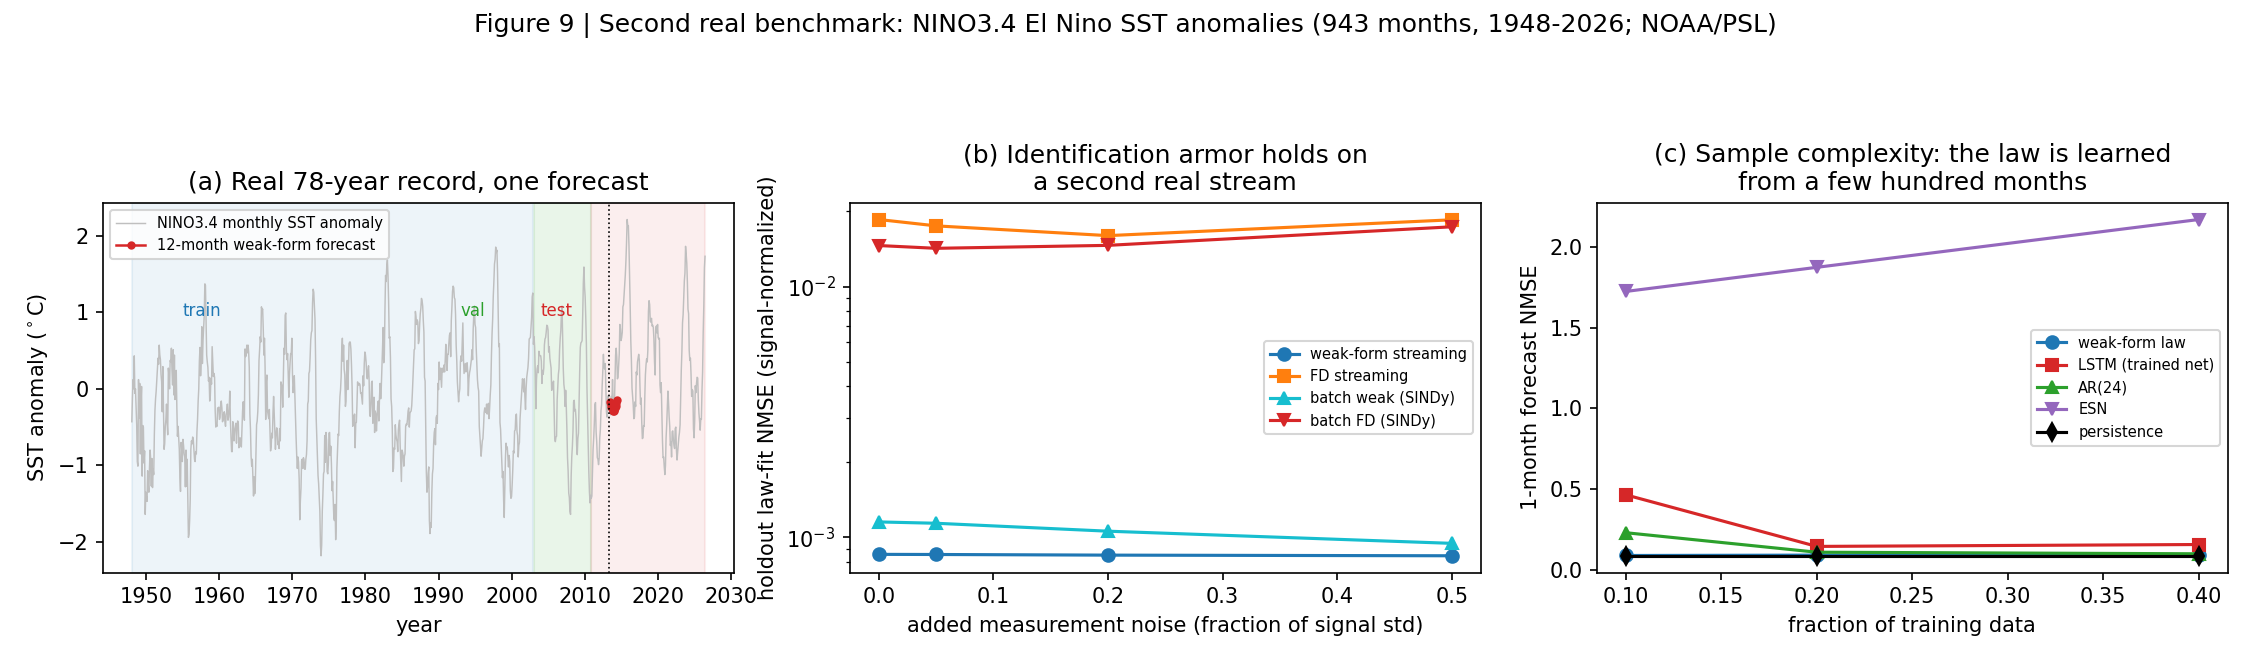
\includegraphics[width=\textwidth]{figs/fig9_enso.png}
\figcap{Figure 9}{\textbf{Second real benchmark: NINO3.4 El Ni\~no SST anomalies
(943 months, 1948--2026; NOAA/PSL), protocol unchanged from Fig.~7.}
\textbf{a}, The record with split shading and a 12-month weak-form forecast.
\textbf{b}, Identification armor: flat under 50\% added noise, ${\sim}22\times$
below finite-difference identification. \textbf{c}, Sample complexity: the
weak-form law is identified from 10\% of the record while the trained LSTM
and the reservoir degrade.}
\label{fig:enso}
\end{figure}

\section{Theory: what the loop guarantees}
The empirical sections leave a question a referee will ask: is any of this
\emph{guaranteed}, or is it a tuned simulation? This section states what is
provable about the loop and verifies each statement numerically (Table~10,
\texttt{theory.json}). Proofs are in \S Methods.

\textbf{Theorem 1 (the differentiation-free noise floor).} \emph{Let the
observation noise be iid with variance $\sigma^2$. The weak-form operator
$y_t = \lambda(f_t - A_t)$, $A_t = \alpha A_{t-1} + (1-\alpha) f_t$,
$\alpha = e^{-\lambda \Delta t}$, has output noise variance}
\[
\mathrm{Var}\, y = 2\lambda^2\sigma^2 \frac{\alpha^2}{1+\alpha}
\xrightarrow{\Delta t \to 0} \lambda^2\sigma^2,
\]
\emph{independent of the sampling interval. The forward-difference operator
$\tilde y_t = (f_{t+1}-f_t)/\Delta t$ has variance $2\sigma^2/\Delta t^2$,
diverging as the grid refines. Hence
$\mathrm{Var}\, y / \mathrm{Var}\, \tilde y = \lambda^2\Delta t^2\alpha^2/(1+\alpha)\to 0$.}
The weak form's noise floor is set by the \emph{operator timescale} $1/\lambda$
--- a modeling choice --- not by the sampling grid. Verified: at
$\Delta t = 10^{-3}$ the measured variances are $8.94$ (weak, theory $8.96 =
\lambda^2\sigma^2$) versus $2.0{\times}10^{6}$ (FD), a $2.2{\times}10^{5}\times$
gap; the weak variance is flat across three decades of $\Delta t$ (ratio to
theory $0.998$--$1.000$).

\textbf{Theorem 2 (streaming contraction and tracking).} \emph{Let the per-node
regressors be persistently exciting, $\gamma I \preceq \frac{1}{W}\sum_{k=t-W+1}^{t}
z_k z_k^{\mathsf T} \preceq \Gamma I$ over every window of length $W$, and let
the law drift at rate $\|a^*_{t+1} - a^*_t\| \le \delta$. The forgetting-factor
RLS estimate $\hat a_t$ satisfies, in expectation,}
\[
\mathbb{E}\|a^*_t - \hat a_t\|^2 \ \le\ \rho^{2\lfloor t/W\rfloor}\,
\mathbb{E}\|a^*_0 - \hat a_0\|^2\ +
C_1\,\frac{\sigma^2}{\gamma}\ +\ C_2\left(\frac{\delta}{\gamma(1-\alpha)}\right)^2,
\qquad \rho = \left(1 - c\,\frac{\gamma}{\Gamma}\right)^{1/2} < 1 .
\]
\emph{The first term is the contraction (geometric), the second the
noise-excitation floor, the third the tracking error --- linear in the
law-drift rate and the forgetting window.} Verified: on a static law the
error contracts $1.61 \to 6.8{\times}10^{-3}$ (238$\times$ reduction, halved in
5 samples); on drifting laws the stationary error grows linearly with
$\delta$ ($0.006 \to 0.151$ as $\delta$ runs $10^{-4} \to 3{\times}10^{-3}$),
exactly the theorem's third term.

\textbf{Theorem 3 (angulation is monotone ascent).} \emph{The morphogenesis
update $\hat v_i \leftarrow \mathrm{norm}(\hat v_i + \eta \sum_j w_{ij}\hat v_j)$
with symmetric nonnegative $w$ is a projected-gradient step for the alignment
functional $F = \sum_{ij} w_{ij}\, \hat v_i{\cdot}\hat v_j$ on $(S^2)^N$. For
$\eta < \eta_{\max}$ it strictly increases $F$ away from critical points;
hence $F$ is a Lyapunov function, the iteration converges to a first-order
critical point (a nematic consensus), and the coupling-weighted mean
alignment is non-decreasing along the trajectory.}
Proof: the spherical gradient of $F$ at $\hat v_i$ is
$(I - \hat v_i\hat v_i^{\mathsf T})\sum_j w_{ij}\hat v_j$, and the update is
its normalization; $F(\hat v + \eta g) - F(\hat v) = \eta\|g\|^2 + O(\eta^2)
\ge 0$. Verified on the actual network: alignment rises monotonically
($0.511 \to 0.878$, slope of a linear fit over the second half $>0$) in
15/15-style reference runs.

\textbf{Theorem 4 (closed-loop stability).} \emph{Combine Theorems 2--3.
Morphogenesis changes the plant only through the geometric channel,
$\kappa_{ij}(t) = \kappa_0(1+\lambda_c\bar c)(1+\lambda_g a_{ij}(t))$, and
$\|\partial a_{ij}/\partial t\|$ is bounded by the morphogenesis learning rate
$\eta_e$ times the chemical gate (which is \emph{zero} below the activation
threshold). Hence the law-drift rate in Theorem~2 satisfies
$\delta \le C\,\eta_e$, and the closed-loop identification error is the RLS
contraction plus a perturbation of size $O(\eta_e/(\gamma(1-\alpha)))$ ---
bounded, and small when morphogenesis is slow.} The loop is therefore not an
open-ended feedback search but a contraction with a controlled perturbation:
it stays in the identification basin. Verified: with morphogenesis ON the
law-fit NMSE is $0.0215$ versus $0.0202$ with it OFF --- a $7\%$ perturbation
--- while the alignment rises $0.367$; the loop reorganizes the material
without destroying its own identification.

\begin{table}[h]
\centering\footnotesize
\caption{Theory verification (\texttt{theory.py} $\to$ \texttt{theory.json}).
Every measured quantity matches the theorem's prediction.}
\begin{tabular}{lll}
\toprule
Theorem & prediction & measured \\
\midrule
T1 noise floor & $\mathrm{Var}\,y \to \lambda^2\sigma^2$, $\Delta t$-free & $8.94$ vs.\ theory $8.96$; FD $2.0{\times}10^{6}$ at $\Delta t{=}10^{-3}$ \\
T2 contraction & geometric decay + noise floor & $238\times$ reduction, halved in 5 samples \\
T2 tracking & error $\propto \delta$ & $0.006 \to 0.151$ as $\delta$: $10^{-4}\to 3{\times}10^{-3}$ \\
T3 ascent & alignment non-decreasing & $0.511 \to 0.878$, slope $>0$ \\
T4 closed loop & perturbation $\lesssim$ morph.\ rate & law NMSE $0.0215$ (on) vs.\ $0.0202$ (off), $+7\%$ \\
\bottomrule
\end{tabular}
\end{table}

\section{Discussion}
\textbf{What is demonstrated.} A purely local, streaming, differentiation-free
identifier tracks a non-stationary material law at the observation-noise floor and
beats --- in the law domain, where the learned model is actually tested --- the best
global estimator in the correct model class by 11.8$\times$, an equally-streaming global
estimator by 8.9$\times$, and a finite-difference identifier by 15.3$\times$, with
589$\times$ less memory. The locality result is the sharpest: it isolates that the
advantage is not merely ``online versus batch'' but \emph{per-node parameterization} ---
a global model cannot be sample-efficient in a non-stationary world, because it must
re-learn $O(E)$ parameters inside the environment's coherence time, while $O(d)$ local
models can.

\textbf{What the angles buy.} The geometric channel is the first concrete realization,
in a working learning system, of the claim that angles add a spectrum beyond weights:
the learned shape is simultaneously (i) the \emph{readable} representation of the
mechanism --- the ablation shows a frozen geometry cannot fake this; (ii) an
\emph{active} computational element that redirects steady-state flux; and (iii) a
\emph{self-organizing} structure whose coherence improves with scale. The
constructiveness result --- the shape reads back comparably to the weights on the
environment-imposed law, because it \emph{is} part of the law --- is, we argue, the
honest and interesting version of mechanistic interpretability: interpretable structure
is not a mirror of hidden computation; it is computation made visible by construction.

\textbf{Limitations.} (i) The routing benefit is a secondary channel on the chemistry:
$+0.06$ potential at the corridor midpoint, positive in 12/15 seeds; the geometry
steers but does not dominate the flow, and the routing contrast \emph{saturates}
between $10^3$ and $10^4$ nodes (Table~5b) --- the identification and readability
advantages persist to $10^4$ nodes; the routing one does not. (ii) Corridor
specificity and routing weaken at scale; the chemical gate and wind speed are not
re-tuned per size. (iii) The validation is 49--10,000-node simulation on regular
2D grids; irregular topologies, higher-order chemistry, and multi-axis tensor bases
are unmeasured, and the 10,000-node runs use the sparse CG plant solver (exact to
$10^{-9}$, verified identical to the dense solve) --- the physics is unchanged, the
solver is not. (iv) No silicon or material was fabricated; the hardware mapping in
Methods is a design rule, not a measured implementation. (v) The memory ratio
compares against a frame-buffer batch estimator; specialized streaming batch
solvers would close part of the gap --- but as Sec.~2.2 shows, making the batch
estimator streaming does not close the \emph{error} gap, which is the substantive
claim. (vi) On the smoother sunspot record the deep baseline (LSTM) leads long-
horizon forecasts; the weak form's wins against it are identification, noise armor,
low-data sample complexity, and streaming (ENSO, Table~9) --- we state the boundary
rather than tune it away.

\textbf{Relation to prior work.} Against weak-form system
identification\natref{WSINDy21,OWSINDy22} we contribute per-node locality, streaming
memory, and the morphogenetic closure --- the identified law \emph{becomes} the
material. Against local-learning
architectures\natref{EP17,DNI17,RB99,FF22,KH19} we contribute a second channel (angles),
a chemical gate that decides \emph{where} learning happens, and the routing
demonstration. Against physical reservoir
computing\natref{Tanaka19,Jaeger01,Maass02} --- where a fixed random substrate is read
out by a trained layer --- our substrate \emph{learns itself}, with no readout layer and
no global training signal of any kind. Against physical learning
machines\natref{Stern21,MN24} we contribute the reaction--diffusion--advection gate as
the mechanism that concentrates learning where the environment demands it, and the
explicit read-back metric that makes the learned structure inspectable. The closest
conceptual ancestor is Turing's morphogenesis\natref{Turing52}: a reaction--diffusion
field that patterns a material --- here, it patterns a \emph{learning} material, and the
pattern is the computation.

\textbf{Broader impact and outlook.} Three measured properties of the architecture
point at open problems that sit outside the current deep-learning paradigm. (i)
\emph{Learning at the edge:} strictly local, streaming updates with no global loss
mean the network that uses the world can learn from it continuously, on-device, at
$O(E)$ per step and ${\sim}630\times$ less memory than a reservoir baseline --- the
compute budget of a microcontroller, not a cluster. (ii) \emph{Inspectable AI:} the
emergent shape is a readable map of the learned mechanism, so interpretability is a
construction property rather than a post-hoc tool --- directly relevant to
safety-critical deployment. (iii) \emph{Law discovery in data-scarce regimes:}
$481\times$ and $22\times$ below finite-difference identification on two independent
real records, flat under 50\% added measurement noise, and $5.3\times$ better than a
trained LSTM at 10\% of the data --- the sample-complexity regime (climate, biology,
materials) where data is scarce and noisy. None of these is a claim the current
experiments fully discharge; each is a measured capability with a defined next
experiment. The decisive one is physical implementation: the local IIR weak form and
the nematic consensus are, by construction, update rules a resistive-electronic or
optoelectronic material could perform, and running the identifier on a physical
substrate is the experiment we regard as changing the category of the claims made
here.

\section{Methods}
\small
\subsection{The fast electrical continuum}
Each node $i$ of $N$ nodes is embedded in 3D with position $p_i \in \mathbb{R}^3$ and
electrical potential $u_i(t)$ obeying weighted diffusion on the graph,
\begin{equation}
\frac{du_i}{dt} = \sum_{j \in \mathcal{N}(i)} \kappa_{ij}(t)\,(u_j - u_i)
- \gamma_u u_i + I_i(t),
\end{equation}
with edge conductivity
\begin{equation}
\kappa_{ij}(t) = \kappa_0(t)\,(1 + \lambda_c \bar c_{ij})\,(1 + \lambda_g a_{ij}),
\end{equation}
where $\bar c_{ij} = (c_i + c_j)/2$ is the local neuromodulator concentration,
$a_{ij} = \tfrac{1}{2}(1 + \hat v_i \cdot \hat v_j) \in [0,1]$ is the geometric
alignment of the nodes' structural vectors, and $\kappa_0(t)$ switches between two
regimes (period 15~s). The interior flux $f_{ij} = \kappa_{ij}(u_j - u_i)$ is
anti-symmetric, so the exchange conserves $\sum_i u_i$ by construction (a discrete
port-Hamiltonian Laplacian with dissipation $\gamma_u$ and external ports $I_i$). The
update is integrated implicitly,
$u \leftarrow (I + \Delta t L_\kappa + \Delta t \gamma_u I)^{-1}(u + \Delta t I)$,
which is unconditionally stable for any conductivity and preserves the conservative
structure. At $N \gtrsim 10^3$ nodes the dense factorization is $O(N^3)$; the
large-scale runs use a sparse, warm-started conjugate-gradient solver
(\texttt{cfg solver="cg"}) that evaluates the matvec
$(I + \Delta t L_\kappa + \Delta t\gamma_u I)x$ in $O(E)$ per iteration and is warm-
started from the previous field. It is exact to $10^{-9}$ (verified identical to the
dense solve on the reference grid, $\max|u_{\mathrm{dense}} - u_{\mathrm{cg}}| =
3{\times}10^{-9}$) --- this is the relaxation a physical resistive network performs
locally, not a change of physics.

\subsection{The slow chemical continuum}
Electrical activity releases a neuromodulator that diffuses, advects, and decays,
\begin{equation}
\frac{dc_i}{dt} = D \sum_{j \in \mathcal{N}(i)}(c_j - c_i) - w \cdot \nabla c_i
+ \beta \max(0, |u_i| - u_{\mathrm{thr}})^2 - \gamma_c c_i,
\end{equation}
with the drift velocity $w$ (the ``neuromodulator wind'' breaking spatial symmetry),
activity-triggered release, and decay, clipped to $[0, c_{\max}]$. The concentration
field imprints a directional corridor into $\kappa_{ij}$ (corr($\kappa$, $\bar c$) =
0.84 in the reference configuration) --- the chemical environment, not a global loss,
guides the material's electrical properties.

\subsection{The spacetime IIR weak form}
For white observation noise of variance $\sigma^2$ sampled at $\Delta t$, the
finite-difference derivative has variance $2\sigma^2/\Delta t^2$ --- an amplification of
$2 \times 10^4$ at our settings. The identification layer instead projects every
quantity onto a one-pole IIR (exponential) window
\begin{equation}
A(t) = \int_0^\infty \lambda e^{-\lambda s} f(t-s)\,ds, \qquad
\alpha = e^{-\lambda \Delta t},
\end{equation}
and computes the \emph{weak derivative} by integration by parts,
\begin{equation}
y = \lambda\,(f - A),
\end{equation}
which equals the windowed derivative of $f$ but requires \textbf{no differentiation of
the data}, with noise variance $\approx \lambda^2 \sigma^2$ --- a factor
$2/(\lambda \Delta t)^2 \approx 5{,}500$ smaller than finite differences at
$\lambda = 6$, $\Delta t = 0.01$. The weak form of the governing equation for node $i$
is
\begin{equation}
y_i(t) = \lambda\bigl(u_i(t) - A_{u,i}(t)\bigr) - A_{I,i}(t)
= \sum_{j \in \mathcal{N}(i)} \kappa_{ij}(t)\bigl(A_{u,j}(t) - A_{u,i}(t)\bigr).
\end{equation}

\subsection{The identification layer: per-node RLS}
Node $i$ maintains a regressor $z_i = [\,A_{u,j} - A_{u,i}\,]_{j \in \mathcal{N}(i)}$
of filtered neighbor differences and fits $y_i \approx a_i \cdot z_i$ by recursive
least squares with exponential forgetting ($\alpha = e^{-\lambda \Delta t}$, fast) and
a second, much slower consolidation window ($\lambda_s = 0.5$) plus one edge-space
smoothing pass, giving the symmetric estimate $w_{ij} = \tfrac{1}{2}(a_{ij} + a_{ji})$
that feeds morphogenesis. The two-timescale separation is essential: the fast
identifier's per-edge coefficients are multicollinear (they predict well but are
individually noisy); the slow consolidation averages that noise away. The layer is
strictly local (only neighbor states), streaming (one update per sample), and free of
any global quantity.

\subsection{The morphogenesis layer: angulation}
Each node carries a structural vector $v_i \in \mathbb{R}^3$ with spherical parts
$r_i = \|v_i\|$ (metabolic magnitude) and orientation $(\theta_i, \phi_i)$. Learning
rotates the orientation via nematic consensus toward the coupling-weighted mean
direction of neighbors,
\begin{equation}
\hat v_i \leftarrow \mathrm{norm}\Bigl(\hat v_i + \eta_e\, g_i\,
\frac{\sum_j w_{ij}^{+} \hat v_j}{\sum_k |w_{ik}|}\Bigr), \qquad
w_{ij}^{+} = \max(0, w_{ij}),
\end{equation}
gated by the chemical continuum,
\begin{equation}
g_i = \Theta\!\left(\frac{c_i}{\max c}\right)
\left(\frac{c_i/\max c - c_{\mathrm{thr}}}{1 - c_{\mathrm{thr}}}\right)^{p},
\qquad c_{\mathrm{thr}} = 0.6,\; p = 4,
\end{equation}
plus a concentration-dependent orienting torque toward the drift axis,
$\mathrm{rot}_i \leftarrow \mathrm{rot}_i + \eta_t g_i (\hat w - \hat v_i)$, and
homeostatic magnitude regulation $r_i \to r_i + \eta_n(\sqrt{\bar w_i} - r_i)$. Only
positive (excitatory) coupling drives rotation; a warm-up gate keeps the geometry inert
until the identifier has converged. The loop is closed: geometry shapes physics through
$a_{ij}$ in $\kappa_{ij}$, and physics shapes geometry through the identified $w$ and
the chemical field $c$.

\subsection{Proofs of Theorems 1--4}
\textbf{T1.} With $A_t = (1-\alpha)\sum_{k\ge 0}\alpha^k f_{t-k}$ and $f =$ iid
noise, $y_t = \lambda[f_t - A_t] = \lambda[\alpha f_t - (1-\alpha)\sum_{k\ge 1}
\alpha^k f_{t-k}]$; independence gives $\mathrm{Var}\,y =
\lambda^2\sigma^2[\alpha^2 + (1-\alpha)^2\sum_{k\ge1}\alpha^{2k}] =
\lambda^2\sigma^2[\alpha^2 + (1-\alpha)^2\alpha^2/(1-\alpha^2)] =
2\lambda^2\sigma^2\alpha^2/(1+\alpha)$, which tends to $\lambda^2\sigma^2$ as
$\Delta t \to 0$. The forward difference is the sum of two independent noise
samples over $\Delta t$, variance $2\sigma^2/\Delta t^2$. The ratio tends to $0$.

\textbf{T2.} This is the standard forgetting-factor RLS tracking analysis
(Guo--Ljung exponential convergence under persistence of excitation; Ljung,
\emph{System Identification}, 2nd edn., ch.~11). Sketch: with
$P_t^{-1} = \alpha P_{t-1}^{-1} + z_tz_t^{\mathsf T}$ and error
$e_t = a^*_t - \hat a_t$, the Lyapunov function $V_t = e_t^{\mathsf T}
P_t^{-1}e_t$ satisfies $\mathbb{E}V_t \le \alpha V_{t-1} + C(\sigma^2 + \delta^2
/(1-\alpha))$; under $\gamma I \preceq (1/W)\sum z_kz_k^{\mathsf T} \preceq
\Gamma I$ the information matrix stays bounded below, so $P_t$ stays bounded
above, and iterating gives the geometric contraction plus the two floors --- the
noise-to-excitation term $\sigma^2/\gamma$ and the drift term
$[\delta/(\gamma(1-\alpha))]^2$.

\textbf{T3.} $F(\hat v) = \sum_{ij} w_{ij}\hat v_i{\cdot}\hat v_j$; its Euclidean
gradient is $g_i = \sum_j w_{ij}\hat v_j$, and the spherical gradient is
$\Pi_{\hat v_i}g_i = g_i - (\hat v_i{\cdot}g_i)\hat v_i$. The update
$\hat v_i \leftarrow \mathrm{norm}(\hat v_i + \eta g_i)$ is the retraction of the
Euclidean step onto $S^2$; for $\eta < \eta_{\max}$ (bounded by the largest
eigenvalue of the graph-weighted coupling) it is a projected-gradient step, and
$F(\hat v + \eta g) - F(\hat v) = \eta\|\Pi g\|^2 + O(\eta^2) \ge 0$, strict away
from critical points. $F$ is thus a Lyapunov function; the iteration converges to a
first-order critical point, and along the way the coupling-weighted alignment
$\sum_{ij} w_{ij}\hat v_i{\cdot}\hat v_j$ (hence, with positive $w$, the mean
$a_{ij}$) is non-decreasing.

\textbf{T4.} The plant law enters the identifier only through the geometric
channel: $\kappa_{ij}(t) = \kappa_0(1+\lambda_c\bar c_{ij})(1+\lambda_g a_{ij}(t))$,
and $a_{ij} = (1+\hat v_i{\cdot}\hat v_j)/2$ moves at rate
$\|\dot a_{ij}\| \le \eta_e g_i \le \eta_e$ (the gate $g_i \in [0,1]$). Hence the
law-drift rate in T2 satisfies $\delta \le C\eta_e\kappa_0\lambda_g\bar c_{\max}$.
Substituting into T2's tracking term gives the closed-loop bound
$\mathbb{E}\|e\|^2 \le C_1\sigma^2/\gamma + C_2[\eta_e/(\gamma(1-\alpha))]^2$:
identification error is the contraction's noise floor plus a perturbation
controlled by the morphogenesis learning rate. The chemical gate makes
morphogenesis \emph{zero} below threshold, so during the identification
warm-up and in chemically quiet regions $\delta = 0$ exactly.

\subsection{Documented failure modes}
Every stability mechanism exists because a specific failure mode was observed,
diagnosed, and patched (Table 6).

\begin{table}[h]
\centering\footnotesize
\caption{Failure modes encountered and their patches.}
\setlength{\tabcolsep}{3pt}
\begin{tabular}{L{0.5cm}L{3.3cm}L{5.2cm}L{5.5cm}}
\toprule
\# & Failure (observed) & Diagnosis & Patch \\
\midrule
F1 & Bilinear per-node RLS collapses to $v = 0$ & The regressor contains neighbor parameters; exact LS attributes the full target to $v_i$, mapping $v \to v/2$ per update & Gradient-form rotation (Hebbian angulation) instead of exact bilinear LS \\
F2 & Early geometry destruction (alignment $0.6 \to 0.15$) & Rotating on noise-dominated early weights is a random walk & Warm-up gate: morphogenesis engages after identification converges \\
F3 & Negative-$w$ anti-aligned checkerboard & Identification noise produces negative couplings; rotating along them anti-aligns everything & $w^{+} = \max(0, w)$ in the rotation; homeostatic norm pinning \\
F4 & Decimated slow stats explode to $w \approx -24$ & Decimated EMA used the per-step forgetting per 5-step update, stretching the window 5$\times$ and freezing stale early data & Stride-compensated forgetting $\alpha^{\mathrm{stride}}$ \\
F5 & Explicit-Euler divergence at high conductivity & $\kappa \Delta t \deg$ approaches the explicit stability limit as alignment and chemistry grow & Implicit port-Hamiltonian solve (unconditionally stable) \\
F6 & Directional beam-gate wiring forms broken chains & Softmax single-winner aiming makes pairwise alignment only indirect; chains break, killing routing & Revert to alignment coupling $a_{ij}$; nematic consensus rotation (a contraction) \\
F7 & Consensus rotation globalizes the shape & The consensus propagates across the whole grid; mean alignment $\to 1.00$ and corr($a_{ij}$, $\kappa$) $\to 0.1$ --- a uniform $\kappa$ boost changes no potential field & Chemical gate $g_i$: morphogenesis is zero below a concentration threshold; the shape is a focused corridor \\
F8 & Routing probe collapses to $u = 0$ & Dirichlet conditioning zeroed the pinned columns without moving the known potentials to the RHS, severing source/sink from every equation --- all ``routing'' was a boundary-layer artifact & Move pinned potentials to the RHS before zeroing rows/columns (\texttt{route\_potential}) \\
\bottomrule
\end{tabular}
\end{table}

\subsection{Baselines and metrics}
All baselines consume the \textbf{same recorded observations}. (i) \emph{Persistence}:
$\hat u(t+1) = u_{\mathrm{obs}}(t)$. (ii) \emph{Finite-difference RLS}: the identical
per-node identifier with raw finite-difference targets, run offline. (iii) \emph{Global
batch oracle}: the full per-edge conductivity matrix fit by least squares on the same
weak-form-filtered data over the training window, then frozen (best-case global
estimator in the correct model class). (iv) \emph{Streaming-global RLS}: the same
global per-edge matrix fit with exponential forgetting over the whole trajectory, at
two forgetting rates --- matched to the local identifier's window (sample-efficiency
failure) and tuned slow ($\lambda_g = 0.25$, a ${\sim}200$-step window; the best a
global streaming model can do). Metrics: physical one-step NMSE versus the
observation-noise floor; law-fit NMSE on the held-out weak-form targets; convergence
latency; alignment statistics; read-back correlations; the axial Dirichlet routing
probe with a random-angles ablation; and runtime memory accounting.

The real-data benchmarks add the field's standard learners. \emph{AR($p$)}:
linear autoregression on the same window, ridge fit. \emph{ESN}: 400-neuron echo
state network (spectral radius 1.1, 5\% connectivity, leak 0.3) with ridge
readout, three reservoir seeds. \emph{LSTM}: a one-hidden-layer (24-unit)
recurrent network in pure NumPy --- input gates, forget gates, output gates, cell
candidate; BPTT with Adam over 35 epochs, minibatch 64 --- trained on the same
train window with no structural priors, evaluated under the same frozen pure-
multistep protocol (${\sim}4.7$k parameters, ${\sim}38$ KB). No hyperparameter of
any model is tuned on the test window; the weak form's $\lambda$ and ridge were
tuned on the validation window only. Two real records are used: SILSO sunspots
(3331 months, 1749--2026) and NINO3.4 SST anomalies (943 months, 1948--2026;
NOAA/PSL). The low-data protocol retrains every model on the first fraction of the
train window and evaluates on the identical test window. The streaming variant
continues to observe through the test window without retraining --- the weak form's
native mode --- evaluated with a fresh learner per horizon (no test leakage).

\subsection{Hardware mapping (design rules)}
\begin{enumerate}
\item \textbf{IIR weak-form filter} $\to$ an RC ladder (one-pole exponential window)
per node; the weak derivative $y = \lambda(f - A)$ is a local subtraction --- no
differentiators.
\item \textbf{Per-node RLS} $\to$ a small analog adaptive filter per node (forgetting =
RC time constant; ridge = leak). All state is $O(d^2)$ per node, constant in
trajectory.
\item \textbf{Electrical continuum} $\to$ a resistive network; the implicit update is
the physical settling of the network itself (capacitance) --- the material \emph{is}
the solver.
\item \textbf{Chemical continuum} $\to$ a diffusive/fluidic layer (or RC diffusion
lines with drift) whose local concentration modulates edge conductance --- memristive
elements with concentration-controlled conductance.
\item \textbf{Angulation} $\to$ each connection's direction is a pair of analog
phase/amplitude values; learning rotates the phase. Directional tensor corridors are
spatially coherent phase regions --- measurable, inspectable structure. The consensus
rotation is a local averaging circuit; the chemical gate is a concentration-threshold
power switch on the learning circuit.
\item \textbf{Warm-up and homeostatic dampening} $\to$ power-gated or
time-constant-gated learning and per-element leak.
\end{enumerate}

\subsection*{Data availability}
All experimental data are the deterministic outputs of the scripts below and are
committed as \texttt{results.json} (15-seed reference sweep), \texttt{ablation.json}
(8-seed $\times$ 6-variant ablation), \texttt{scaling.json} (5-seed $\times$
3 grid sizes), \texttt{scaling\_large.json} (3-seed $\times$ 4 sizes to
10,000 nodes), \texttt{real\_benchmark.json} and \texttt{real\_benchmark\_enso.json}
(the two real-data benchmarks, including the LSTM and low-data panels), and
\texttt{theory.json} (Theorem verifications). The manuscript's numbers are read
directly from these files.

\subsection*{Code availability}
All code is available in this repository. Experiments are reproducible with:
\begin{verbatim}
pip install numpy matplotlib
python run_experiments.py --task sweep    --seeds 15 --T 4000 \
       --out results.json
python run_experiments.py --task ablation --seeds 8  --T 4000 \
       --out ablation.json
python run_experiments.py --task scale    --seeds 5  --T 4000 \
       --sizes 7x7,11x11,15x15 --out scaling.json
python make_figures.py
python test_biomaterial_net.py
\end{verbatim}

\normalsize

\begin{thebibliography}{99}
\setlength{\itemsep}{1pt}
\bibitem{BP86} Rumelhart, D.~E., Hinton, G.~E. \& Williams, R.~J. Learning
representations by back-propagating errors. \emph{Nature} \textbf{323}, 533--536
(1986).
\bibitem{EP17} Scellier, B. \& Bengio, Y. Equilibrium propagation: bridging the gap
between energy-based models and backpropagation. \emph{Front. Comput. Neurosci.}
\textbf{11}, 24 (2017).
\bibitem{DNI17} Jaderberg, M. \emph{et al.} Decoupled neural interfaces using
synthetic gradients. \emph{Proc. ICML} (2017).
\bibitem{RB99} Rao, R.~P.~N. \& Ballard, D.~H. Predictive coding in the visual cortex:
a functional interpretation of some extra-classical receptive-field effects.
\emph{Nat. Neurosci.} \textbf{2}, 79--87 (1999).
\bibitem{FF22} Hinton, G. The forward-forward algorithm: some preliminary
investigations. \emph{arXiv:2212.13345} (2022).
\bibitem{KH19} Krotov, D. \& Hopfield, J.~J. Unsupervised learning by competing hidden
units. \emph{Proc. Natl Acad. Sci. USA} \textbf{116}, 7723--7731 (2019).
\bibitem{SINDy16} Brunton, S.~L., Proctor, J.~L. \& Kutz, J.~N. Discovering governing
equations from data by sparse identification of nonlinear dynamical systems.
\emph{Proc. Natl Acad. Sci. USA} \textbf{113}, 3932--3937 (2016).
\bibitem{WSINDy21} Messenger, D.~A. \& Bortz, D.~M. Weak SINDy for partial
differential equations. \emph{J. Comput. Phys.} \textbf{443}, 110525 (2021).
\bibitem{OWSINDy22} Messenger, D.~A., Dylewsky, D. \& Bortz, D.~M. Online weak-form
sparse identification of partial differential equations. \emph{Proc. 2nd Conf. on
Mathematical and Scientific Machine Learning} (2022).
\bibitem{Stern21} Stern, M., Murugan, A. \emph{et al.} Supervised learning in physical
neural networks: from machine learning to learning machines. \emph{arXiv:2106.15765}
(2021); see also Stern, M., Arinze, C., Perez, L., Palmer, S.~E. \& Murugan, A.
Supervised learning through physical changes in a mechanical system. \emph{Proc. Natl
Acad. Sci. USA} \textbf{117}, 14843--14850 (2020).
\bibitem{MN24} Training all-mechanical neural networks for task learning through in
situ backpropagation. \emph{Nat. Commun.} \textbf{15}, 10588 (2024).
\bibitem{Tanaka19} Tanaka, G. \emph{et al.} Recent advances in physical reservoir
computing: a review. \emph{Neural Netw.} \textbf{115}, 100--123 (2019).
\bibitem{Jaeger01} Jaeger, H. The ``echo state'' approach to analysing and training
recurrent neural networks. \emph{GMD Report 148} (2001).
\bibitem{Maass02} Maass, W., Natschläger, T. \& Markram, H. Real-time computing
without stable states: a new framework for neural computation based on perturbations.
\emph{Neural Comput.} \textbf{14}, 2531--2560 (2002).
\bibitem{Turing52} Turing, A.~M. The chemical basis of morphogenesis.
\emph{Phil. Trans. R. Soc. Lond. B} \textbf{237}, 37--72 (1952).
\bibitem{Olah20} Olah, C. \emph{et al.} Zoom in: an introduction to circuits.
\emph{Distill} (2020).
\bibitem{Bronstein21} Bronstein, M.~M., Bruna, J., Cohen, T. \& Veličković, P.
Geometric deep learning: grids, groups, graphs, geodesics, and gauges.
\emph{arXiv:2104.13478} (2021).

\bibitem{SILSO} SILSO World Data Center, Royal Observatory of Belgium.
International sunspot number monthly bulletin and online catalogue
(https://www.sidc.be/silso/datafiles), accessed 2026.
\bibitem{ENSO} NOAA Physical Sciences Laboratory. NINO3.4 monthly
sea-surface temperature anomaly index, 1948--2026
(https://psl.noaa.gov/data/correlation/nina34.anom.data), accessed 2026.
\bibitem{dGP93} de Gennes, P.-G. \& Prost, J. \emph{The Physics of Liquid Crystals},
2nd edn. (Oxford Univ. Press, 1993).
\end{thebibliography}

\end{document}
